\documentclass[11pt,a4paper]{article}

% --- Packages for Genome Medicine-style typesetting -----------------------
\usepackage[utf8]{inputenc}
\usepackage[T1]{fontenc}
\usepackage[english]{babel}
\usepackage[margin=2.5cm]{geometry}
\usepackage{setspace}
\usepackage{graphicx}
\usepackage{float}
\usepackage[font=small,labelfont=bf,labelsep=period,justification=justified,singlelinecheck=false]{caption}
\usepackage{booktabs}
\usepackage{amsmath}
\usepackage{amssymb}
\usepackage{siunitx}
\usepackage{xcolor}
\usepackage{titlesec}
\usepackage[sort&compress,numbers]{natbib}
\usepackage{hyperref}
\hypersetup{colorlinks=true, linkcolor=black, citecolor=blue, urlcolor=blue}

\setstretch{1.3}
\titleformat{\section}{\large\bfseries}{\thesection}{0.6em}{}
\titleformat{\subsection}{\normalsize\bfseries}{\thesubsection}{0.6em}{}
\renewcommand{\abstractname}{}  % use custom structured abstract

\title{\bfseries\LARGE Chemical reachability limits mutagen-based TKI-resistance screens}

\author{Michele Ronco$^{1,*}$ \\[0.3em]
\small ORCID: \href{https://orcid.org/0000-0002-2160-2452}{0000-0002-2160-2452} \\[0.3em]
\small $^{1}$European Commission Joint Research Centre, Ispra, Italy \\
\small $^{*}$Correspondence: \href{mailto:michele.ronco@ec.europa.eu}{michele.ronco@ec.europa.eu}}

\date{}

\begin{document}
\maketitle

% ============================================================================
% STRUCTURED ABSTRACT  (BMC Genome Medicine house style)
% ============================================================================
\section*{Abstract}

\paragraph{Background.}
Preclinical Ba/F3 mutagenesis screens are a first line of evidence for
predicting kinase-inhibitor resistance, and their hit lists shape
resistance panels for KRAS G12C, ALK, and MET inhibitors. Every mutagen
in use has a non-uniform substitution spectrum, and whether that
chemistry limits which resistance variants a screen can find, or only
reorders them, has not been audited against a chemistry-free baseline.

\paragraph{Methods.}
We separate a screen's expected output into a supply term, from codon
tables and each mutagen's six-class spectrum, and a selection term,
from chemistry-free deep mutational scans of KRAS G12C, ALK, and MET:
$P(v) \propto S_{\mathrm{mutagen}}(v) \cdot \exp(\beta\sigma(v))$. We
test supply by enumerating what each chemistry cannot reach, and
selection by asking whether supply improves the ranking of the hits
four retrospective screens reported.

\paragraph{Results.}
Chemistry acts as a reachability threshold, not a ranking weight. Base
editors, which produce only two of the six substitution classes, cannot
supply seven of the twelve KRAS G12C panel variants or most of each ALK
drug's top-ranked variants. A second limit binds every
single-nucleotide mutagen: roughly three-quarters of each MET
inhibitor's top 100 priorities need two or more nucleotide changes.
Past that threshold supply does not improve the ranking on any anchor,
and mutagens with very different spectra recover ALK variants at
indistinguishable rates. Two MET screens sharing one mutagen and one
cell line gave different class compositions ($P = 0.029$), so
composition follows the drug, though clone counts within a single codon
did track supply.

\paragraph{Conclusions.}
The deliverable is the reachability inventory: which resistance
variants a mutagen-and-drug pair cannot produce, enumerable from codon
tables and a published spectrum before the screen runs. Reweighting the
output afterward does not recover them, so chemistry belongs in a
screen's design, not in its interpretation.


\paragraph{Keywords.}
Preclinical resistance screens; mutational signatures; ENU; Mutazyme;
base editing; prime editing; deep mutational scanning; KRAS G12C;
sotorasib; adagrasib; ALK; alectinib; lorlatinib; neladalkib; chemistry
bias.

% ============================================================================
% BACKGROUND
% ============================================================================
\section{Background}

Preclinical mutagenesis of Ba/F3 cells transduced with an
oncogenic kinase is the standard first-line assay for predicting the
resistance variants that will emerge in patients treated with a given
tyrosine-kinase inhibitor (TKI)
\citep{warmuth2007,doi2022,koga2021,tang2022boehringer}. The assay was
first developed for BCR-ABL1 and has since been applied to the resistance
landscapes of ALK, FLT3, EGFR, KIT, FGFR, MET, ROS1, and KRAS G12C
\citep{bradeen2006,azam2003,doi2022,takei2025,tang2022boehringer,tanaka2021,awad2021,feng2022,oh2026,tiedt2011,keddy2022}.
Its appeal is that the output ranks variants by relative resistance
in cells, and that the top-ranked variants have reproducibly matched
the mutations that later appeared on ctDNA liquid-biopsy panels of relapsed patients
\citep{tanaka2021,awad2021}.

The assay rests on a mutagenesis step, and that step is almost always
done with a chemistry-biased mutagen. In current (2024--2026) practice,
an industry screen of the fourth-generation ALK TKI neladalkib (NVL-655)
used ENU \citep{tangpeerachaikul2025}; a next-generation ALK TKI panel
screen covering alectinib, lorlatinib, zotizalkib, and neladalkib used
error-prone PCR \citep{takei2025}; and a recent KRAS G12C resistance
screen against adagrasib and the RAS(ON) tri-complex inhibitors used a
combination of CRISPR cytosine and adenine base editors
\citep{diaz2025}.
Each of these chemistries supplies the six pyrimidine substitution
classes (C$>$A, C$>$G, C$>$T, T$>$A, T$>$C, T$>$G) at distinct
probabilities: ENU is dominated by T$>$C and T$>$A, Mutazyme II by
C$>$T, and base editing is restricted by design to C$>$T and T$>$C.
The resulting six-class supply pattern is distinct for every chemistry.
Because the hit list these screens produce is what informs resistance
panels and treatment-sequencing decisions, a variant the chemistry
cannot reach is not merely absent from an experiment. It is absent from
the evidence base that clinicians and trial designers consult, and no
amount of sequencing depth will recover it.
We quantify two things. First, which reported resistance variants each
chemistry cannot produce in a single nucleotide step, separating those
observed in patients from those observed only in an accompanying
\textit{in vitro} scan. Second, for the variants it can produce,
whether their ranking differs from the chemistry-free one.

Chemistry bias in mutagen output is not a new observation. The
Mutazyme II spectrum is quantified in \citep{doi2022}'s supplement,
ENU's class preferences are compiled in \citep{arnold2012}, the
industry neladalkib poster itself states that ENU ``has mutational
bias'' and that this is ``a potential limitation of this assay''
\citep{tangpeerachaikul2025}, and a Hamming-distance-1 reachability
filter has been applied case-by-case to specific EGFR variants
\citep{wang2025}. Rather than claiming a novel bias, this work
systematizes that filter across mutagens, genes, and drugs, anchors
it in chemistry-free atlases, reports it prospectively with
per-variant codon-level provenance, and benchmarks it against both
the $\sigma$-alone and the supply-alone nulls.

Two recent publications supply the missing baselines
(Table~\ref{tab:current-practice}, bottom two rows). A Twist Biosciences
synthetic saturation mutagenesis library \citep{feng2022} produced every
single-amino-acid substitution of KRAS G12C in a chemistry-free pool,
and scored each variant under sotorasib and adagrasib in NCI-H358 cells;
in parallel, a prime-editing atlas \citep{oh2026} generated 3,208
single-nucleotide variants across the ALK kinase-domain locus (2,953
coding SNVs covering the kinase domain plus 255 flanking intronic and
splice-site variants) in H3122
ALK$+$ non-small-cell lung cancer cells and scored each under alectinib,
lorlatinib, and zotizalkib. In both studies, library construction is
decoupled from mutagen chemistry, so the measured drug-selection score
for each variant can be read as the fitness ground truth $\sigma(v)$
against which chemistry-biased screens can be compared. Several further
chemistry-free atlases, independent of this work's two case studies,
extend the template to other kinases. For \textit{MET}, a kinase-domain
DMS \citep{estevam2024}: a Twist-synthesized library of 5,764
substitutions scored in Ba/F3 against eleven \textit{MET} inhibitors
spanning type I, I$\tfrac{1}{2}$, II, and III mechanistic classes. For
\textit{EGFR}, two atlases: a full-length EGFR DMS \citep{hayes2024} of
$\sim$22{,}500 variants across all 1{,}210 residues scored in the
EGFR-dependent human lung cancer line PC9 against erlotinib, afatinib,
dacomitinib, and osimertinib (with clinical validation in two
glioblastoma patients bearing EGFR G598V); and an EGFR L858R
kinase-domain DMS \citep{wang2025}, a $\sim$17{,}000-variant library
built by mutagenic PCR with degenerate codon primer pools (explicitly
reporting negligible transition/transversion bias) and scored in Ba/F3
against osimertinib, BLU-945, and seven additional EGFR TKIs. Together
with the KRAS G12C and ALK atlases, these chemistry-free DMS atlases
demonstrate that chemistry-decoupled DMS of a kinase domain against a
clinical inhibitor panel is a reproducible experimental template across
kinases and library-construction routes (Twist synthesis, prime editing,
MITE-based oligonucleotide tiling, degenerate-codon mutagenic PCR), now
extending beyond the KRAS G12C and ALK cases we analyze here.

We decompose a chemistry-biased screen's expected output as a product
\begin{equation}
    P(v) \;\propto\; S_{\mathrm{mutagen}}(v) \cdot E(v),
\label{eq:decomp}
\end{equation}
with $S_{\mathrm{mutagen}}(v)$ the probability that the given mutagen
produces the variant $v$ in one single-nucleotide step from the
wild-type codon, and $E(v) = \exp(\sigma(v))$ the drug-induced
enrichment factor, with $\sigma(v)$ the drug-selection score read
from the atlas on a log scale. On the log scale,
\begin{equation}
    \log \hat P(v) \;=\; \log S_{\mathrm{mutagen}}(v) \,+\, \beta \sigma(v),
\label{eq:decomp2}
\end{equation}
with $\beta$ absorbing any scaling between the atlas's reported units
and $\ln E$. For the ALK atlas, $\sigma(v)$ is the Oh atlas Resistance
score reported in log$_2$ units; we work in those units directly
(rankings are invariant to the log-base choice, which only rescales
$\beta$). For the KRAS G12C atlas we treat the Z-score as a
dimensionless selection score. All quantitative rank shifts are
bracketed by a $\beta$-sensitivity interval over $\beta \in [0.25, 4]$
in Results.
Some variants have $S_{\mathrm{mutagen}}(v) = 0$, and the two reasons
differ in kind. When the required substitution class lies outside the
mutagen's chemistry, as with the four classes a cytosine and adenine
base-editor pair cannot write, the rate is exactly zero and no library
depth recovers the variant. When the wild-type codon is more than one
nucleotide away, the one-step rate is zero but the multi-step rate is
not, so the variant is suppressed rather than forbidden; we quantify
that suppression in \S\ref{sec:two-hit} instead of asserting
impossibility. Both cases are identified without any dependence on
$\beta$.

Here we apply this decomposition across two case studies. We lead with
KRAS G12C, where the inhibitor pipeline is in active development and the
predictions are forward-looking: we show that two of twelve variants in a
composite resistance panel (patient cohort \citep{awad2021}, case report
\citep{tanaka2021}, and the accompanying \textit{in vitro} deep
mutational scan \citep{awad2021}) lie outside one-step reach from
the wild-type KRAS codon, that several more are chemistry-under-counted
by current ENU and base-editing screens, and that the previously
unidentified Y96D case-report variant \citep{tanaka2021} is precisely
of the kind our framework predicts should be absent or deeply buried in
standard ENU/Mutazyme screens. We follow with ALK, where five of the
six published Mutazyme-with-alectinib resistance mutations
\citep{doi2022} are class-forced and all five land in the
Mutazyme-simulated top-120 of the chemistry-free atlas (three in the
top-20), as the primary retrospective validation anchor. The framework itself is
independent of the three atlases we use for calibration; we expect it to
apply to any current or future chemistry-biased screen whose mutagen's
substitution spectrum is measured.

% ============================================================================
% METHODS
% ============================================================================
\section{Methods}

\subsection{Datasets}

\paragraph{KRAS G12C saturation mutagenesis atlas.}
Average Z-scores for sotorasib and adagrasib across the KRAS G12C protein
(positions 2--189) were extracted from Table S1 of the published Twist
Biosciences synthetic saturation mutagenesis atlas \citep{feng2022}.
The 10-page tables were parsed from the supplementary PDF with
\texttt{pdfplumber} 0.11.10. The parser enforced that the amino-acid
wild-type at each position matched both the KRAS-4A reference and the
blank-cell pattern in both the sotorasib and adagrasib blocks. 3,567
variants were recovered per drug, with 188 of 188 positions covered.
Position 12 is encoded by the G12C-mutant codon TGT in the library.

\paragraph{ALK saturation mutagenesis atlas.}
Resistance scores for alectinib, lorlatinib, and zotizalkib, together with
fitness scores in the untreated condition, were extracted from Table S2
of the published prime-editing atlas \citep{oh2026}, which reports scores
for 3,208 single-nucleotide variants across ALK residues 1058--1388 of
NM\_004304.5, spanning the ALK kinase domain (UniProt 1116--1392) plus
flanking exon-boundary and intronic positions. Of these, 2,953 are coding (2,173
missense, 665 synonymous, 115 nonsense) and 255 are intronic (149) or
splice acceptor/donor (106); the chemistry-free rankings reported here
are computed over the 2,953 coding SNVs after aggregation to the
amino-acid level. Drug-selection scores are taken directly from the
atlas's Resistance score, $\sigma_{\mathrm{drug}}(v) =
\text{Resistance}(v)$, with amino-acid-level aggregation by mean over
all synonymous SNV routes to the same amino-acid change. Per the
atlas Methods \citep{oh2026}, the Resistance score is itself a
log fold change comparing drug-treated to untreated cells at the same
timepoint ($D10$), so intrinsic variant fitness is already divided out
by the common untreated-$D10$ denominator; the atlas's separately
reported Fitness score is an orthogonal time-course quantity
($\log(\text{untreated}_{D10}/D0)$) used by the atlas authors to
classify variants on a 2D (Resistance, Fitness) plane
(``canonical''~/~``drug-addiction-like''~/~``driver-like''). The two
scores are empirically near-orthogonal across missense variants
($|r| < 0.05$ for all three drugs); subtracting Fitness from
Resistance would therefore double-correct and systematically bias
rankings against driver-like variants and in favor of
drug-addiction-like variants. We use Resistance alone.

\paragraph{KRAS G12C and ALK resistance panels.}
The KRAS G12C resistance panel comprises 12 single-amino-acid variants
drawn from the clinical and preclinical literature on sotorasib and
adagrasib resistance: six patient-observed variants (Y96C, H95D, H95Q,
H95R, R68S from a sotorasib-resistance clinical cohort \citep{awad2021};
Y96D from an adagrasib-resistance case report \citep{tanaka2021}) and
six variants reported in the accompanying \textit{in vitro} deep
mutational scan \citep{awad2021} at codons 8, 12, 68, 95, and 96 (C12F,
V8L, V8M, R68L, R68M, Y96H). Per-variant provenance is given in
Supplementary Table~S1. We refer to this composite set as the
``KRAS G12C resistance panel'' throughout and flag patient-observed
versus preclinical-scan origin where the distinction affects
interpretation. The ALK resistance panel comprises the single-amino-acid
alectinib-, lorlatinib-, and zotizalkib-/neladalkib-resistance variants
reported in \citep{doi2022,takei2025}, used as the retrospective
validation anchor; per-variant provenance is in Supplementary Table~S1.

\paragraph{Retrospective validation set (three ALK screens).}
The retrospective validation in \S\ref{sec:retrospective} and Figure~4
assembles the published variant calls from three preclinical ALK
TKI resistance screens: a Mutazyme II alectinib Ba/F3 screen
\citep{doi2022} (six single-mutation variants, excluding silent
passengers and the I1171S sub-variant of the I1171N/T/S compound call);
an ePCR neladalkib compound screen on an I1171N fixed-V1 background
\citep{takei2025} (five V2 compound partners reported at 500~nM
neladalkib: L1256F, E1129V, E1129K, C1156Y, T1151R); and an industry
ENU screen across alectinib, lorlatinib, and neladalkib
\citep{tangpeerachaikul2025} (thirteen aggregate single-amino-acid
variants: I1171N/S/T, F1174C/V, V1180L, T1151K/R, E1129K, R1192P,
L1196M, G1269A, G1202R). The industry-screen variant list is aggregated
across the three drug arms as the primary report does not disaggregate
by arm. For each variant we compute the reachability class, the
mutagen's class rate from the mutagen's spectrum (Mutazyme II from the
Supplementary NGS of \citep{doi2022}; ENU from \citep{arnold2012}),
and the prime-editing atlas chemistry-free and simulated ranks. Because the prime-editing atlas does not include neladalkib,
the two neladalkib arms use zotizalkib as a
4th-generation ALK TKI proxy for the $\sigma$ term; this is flagged in the
figure and in the derived data file
\texttt{retrospective\_validation.csv}. R1192P falls outside the
atlas's residue window (1058--1388) and is reported as unanchored.

\subsection{Codon tables}

The ALK NM\_004304.5 codon table was assembled from ClinVar variant
records anchored to NM\_004304.5 at each residue reported in the ALK
resistance panel \citep{doi2022,takei2025,oh2026}, and cross-checked
against the EML4-ALK v1 wild-type CDS in the ALK atlas supplement.
The KRAS-4A NM\_033360.4 codon table was reconstructed from the canonical
protein sequence (verified against the blank-cell pattern in the KRAS
atlas table) and ClinVar-anchored at the resistance-panel residues
(V8, G12/C12, S17, Q61, R68, H95, Y96). The 4A-specific hypervariable
region (positions 151--189) was placed by consensus and is not
individually ClinVar-verified, but this region is not involved in the
resistance panel. Both tables are distributed as YAML files with
per-residue \texttt{verified\_by} annotations.

\subsection{Mutagen substitution spectra}

The Mutazyme II spectrum is taken from the supplementary NGS of the
untreated library in \citep{doi2022}. The ENU nominal spectrum is the
compilation \citep{arnold2012} of ENU DNA-adduct conversion
frequencies across published mouse germline mutagenesis studies
\citep{arnold2012}, re-expressed in the six-class pyrimidine
convention. That compilation is phenotype-ascertained: its 587
substitutions are the ones that produced a scorable phenotype in
viable mice, so they have passed both an embryonic-viability filter
and a phenotype-detection filter, and they come from mouse germline
rather than from a Ba/F3 culture. Both differences push in unknown
directions. No pre-selection six-class spectrum measured on an
\emph{in vitro} ENU-treated mammalian library exists in the published
literature, and we were unable to locate one. We therefore use this
compilation as a nominal reference rather than as a calibrated
pre-selection spectrum, we report its sensitivity wherever it enters a
quantitative claim, and \S\ref{sec:retrospective} tests it against the
one \emph{in vitro} ENU output we can observe and finds it
inconsistent. The base-editing nominal spectrum assigns equal mass
to C$>$T and T$>$C and zero to the other four classes, modeling
a 1:1 CBE:ABE mix at the editable positions. The uniform
chemistry-free baseline assigns 1/6 to each of the six classes.
All spectra are stored as six-element vectors summing to~1 and
pass a validation that enforces non-negativity, class completeness,
and tolerance of~5\% on the sum.

\subsection{Class-forced classification}

For each (wild-type amino acid, mutant amino acid, wild-type codon)
triple, we enumerated the single-nucleotide-variant routes from the
wild-type codon to any codon encoding the mutant amino acid, and
assigned each route to one of the six pyrimidine substitution
classes using the standard reverse-complement convention. A
(wild-type, mutant) pair is \emph{reachable in one nucleotide}
if at least one SNV route exists, and \emph{class-forced} if every
such route belongs to the same pyrimidine class. The enumeration
is performed per-codon when the wild-type codon is known;
otherwise it is performed over every synonymous codon encoding
the wild-type amino acid and the result is reported as class-forced
only when every codon's routes agree on a single class.

\subsection{Decomposition and ranking}

For each class-forced variant $v$ with forced class $c(v)$ and
drug-selection score $\sigma_{\mathrm{drug}}(v)$ from the chemistry-free
atlas, the simulated preclinical log-score under mutagen $m$ follows
Eq.~\ref{eq:decomp2} at $\beta = 1$:
$\log \hat{P}_{\mathrm{simulated}}(v, m, \mathrm{drug}) =
\log S_m(c(v)) + \sigma_{\mathrm{drug}}(v)$, and the chemistry-free
log-score is $\log \hat{P}_{\mathrm{chemfree}}(v, \mathrm{drug}) =
\sigma_{\mathrm{drug}}(v)$. Rank-shift point estimates throughout
Results are reported at $\beta = 1$ and bracketed by intervals over
$\beta \in [0.25, 4]$ to make the selection-scale dependence explicit. Variants are ranked in decreasing order
under each score; the ``rank shift'' is $\mathrm{rank}_{\mathrm{simulated}}
- \mathrm{rank}_{\mathrm{chemfree}}$. A positive rank shift means
the mutagen under-counts the variant relative to the chemistry-free
baseline; a negative shift means it over-counts.

Figure~3B reports the top-$K$ recovery curve of each (gene, drug, mutagen)
combination against the chemistry-free ground truth. For each $K \in [1, N]$
with $N$ the class-forced saturation-atlas size, we compute
\begin{equation}
    \mathrm{recovery}(K; m, \mathrm{drug})
    \;=\; \frac{\big|\,\mathrm{top}_K(\log \hat{P}_{\mathrm{simulated}})
          \,\cap\, \mathrm{top}_K(\log \hat{P}_{\mathrm{chemfree}})\,\big|}{K}
    \,.
\end{equation}
Variants with $S_m(c(v)) = 0$ (chemistry-unreachable under $m$) are retained
at a tied-bottom simulated rank by substituting $S_m \to 10^{-6}$ before
log-transforming, so that recovery reflects both within-coverage ranking
distortion and coverage loss across unreachable variants. The chemistry-free
reference curve (Twist \citep{feng2022} for KRAS G12C, prime editing
\citep{oh2026} for ALK) is identically $y = 1$ by construction because the
uniform class supply $S_m \equiv 1/6$ makes $\log \hat{P}_{\mathrm{simulated}}$
differ from $\log \hat{P}_{\mathrm{chemfree}}$ by an additive constant and
preserves the ranking. Curves in Figure~3B are smoothed with a rolling
5-point median to tame small-$K$ noise without erasing the underlying
step structure.

\subsection{Library-depth detection probability}
\label{sec:p-detect}
The decomposition in Eq.~\ref{eq:decomp} is a one-shot supply model.
Real screens sample a library of $N$ cells with per-base mutation rate
$\mu$, and under drug selection a single resistant clone can expand to
detection. The probability that a given variant $v$ has at least one
carrier in a library of size $N$ is
$P_{\mathrm{detect}}(v) \approx 1 - \exp\!\big(-N\,\mu\,S_m(c(v))\,r(v)\big)$,
with $r(v)$ the number of single-nucleotide routes from the wild-type
codon to $v$. For a Ba/F3 library of $N = 10^7$ cells and
$\mu \sim 10^{-4}$ per base per round, $P_{\mathrm{detect}}$ saturates
near 1 for any supplied class above $\sim 10^{-4}$. Every class in
every chemical spectrum used here clears that bound, including ENU's
C$>$G at $2\times 10^{-3}$. Rank-shift predictions therefore apply in
the depth-limited regime, and at practical library depth the binary
distinction $S = 0$ versus $S > 0$ is the operational one. That
distinction is where the reachability results of this paper bind
regardless of $\beta$: exactly for the four classes base editing
cannot write, and to within the two-order suppression computed in
\S\ref{sec:two-hit} for the two-step variants R68L and V8M.

\subsection{Benchmark against null rankings}
\label{sec:benchmark}
For each retrospective anchor (Doi et al.\ 2022 ALK Mutazyme $\times$
alectinib \citep{doi2022}; Tangpeerachaikul et al.\ 2025 industry
ALK ENU aggregate \citep{tangpeerachaikul2025}; Awad et al.\ 2021
KRAS G12C clinical cohort under Mutazyme-simulated sotorasib and
adagrasib \citep{awad2021}), we compute three rankings over the class-forced universe
of the relevant atlas: $\sigma$ alone (chemistry-free); the framework
$\log S + \sigma$; and supply alone $\log S$. For each ranking we report
top-10, top-50, and top-100 recall, and AUROC
(Table~\ref{tab:benchmark}). Permutation p-values for the
framework-minus-$\sigma$-alone top-100 recall gain are computed by
shuffling the \emph{forced\_class} labels across
variants and recomputing the framework ranking 5{,}000 times with a
fixed seed (\texttt{numpy} rng seed 20261013); the empirical two-sided
p-value is $(\sum \mathbb{1}\{\lvert\text{null gain}\rvert \geq
\lvert\text{observed gain}\rvert\} + 1) / (n_{\mathrm{iter}} + 1)$.

These anchors are small, so we also report the resolution of the
permutation test. Recall at $n$ observed hits moves only in units of $1/n$,
which sets a floor on any observable effect, and we take the 97.5th
percentile of the permutation null's absolute gain as the smallest
gain that would reach two-sided significance. Both quantities appear
in Table~\ref{tab:benchmark}. A non-significant $p$ above that
threshold bounds the chemistry term's contribution; it is not evidence
that the contribution is zero.
The Oh et al.\ prime-editing atlas does not include neladalkib, so
for the industry anchor (R10) we proxy $\sigma$ by each of alectinib,
lorlatinib, and zotizalkib in turn. Table~\ref{tab:benchmark} reports
all three proxy results; no proxy gives a framework gain over
$\sigma$-alone that reaches conventional significance.

The agreement between any ranking and the atlas's true $\sigma$ is
bounded by the atlas's own replicate-level reproducibility. The Oh
2026 \citep{oh2026} atlas reports replicate Pearson $r = 0.67$--$0.72$
at SNV level across the three drugs; by Spearman--Brown, the
two-replicate reliability is $\approx 0.82$, so the maximum attainable
correlation between any model's ranking and the underlying resistance
score is $\sqrt{0.82} \approx 0.91$. Top-$K$ overlap ceilings sit
strictly below this correlation ceiling. The 63\%--72\% top-100
recovery for the SNV mutagens reported here therefore cannot be read
as a quantitative deficit of the biased chemistries without reference
to this ceiling; a formal rep-vs-rep top-$K$ ceiling requires access
to the per-replicate atlas scores, which are not released in Table~S2
and are deferred to a follow-up when the authors' repository is
available.

\subsection{Why hit-class composition needs a post-selection null}
\label{sec:class-test}
A screen's reported variants have passed drug selection, so their
substitution-class composition is a post-selection quantity. Comparing
it with the mutagen's pre-selection spectrum attributes to supply any
class enrichment that selection produced. We therefore evaluate an
observed count of $k$ hits of class $c$ in $n$ hits against five
nulls for $\pi(c)$, the probability that a hit belongs to class $c$:

\begin{description}\itemsep2pt
\item[N0, raw spectrum.] $\pi(c) = S_{\mathrm{mutagen}}(c)$. This is
  the comparison that ignores selection.
\item[N1, supply $\times$ composition.] $\pi(c) \propto
  S_{\mathrm{mutagen}}(c)\, n_c$, with $n_c$ the number of class-forced
  atlas variants in class $c$. Corrects for unequal class sizes only.
\item[N2, selection only.] $\pi(c)$ is the share of class $c$ among the
  top-$N$ $\sigma$-ranked class-forced variants ($N = 50, 100, 200$),
  with no supply term. This is the composition a chemistry-free screen
  would report.
\item[N3, model-implied.] $\pi(c) \propto \sum_{v \in c}
  S_{\mathrm{mutagen}}(c)\,\exp(\beta\sigma(v))$, that is,
  Eq.~\ref{eq:decomp2} used as its own null. Under the hypothesis that
  the reference spectrum describes the library, N3 is the hit-class
  distribution the framework predicts.
\item[N4, atlas composition.] $\pi(c) = n_c / \sum_{c'} n_{c'}$, the
  share of class $c$ among all class-forced atlas variants. Drops
  supply and selection both, leaving only how many variants each class
  contains.
\end{description}

N3 is the test of the spectrum; N2 is the test of whether chemistry
enters at all; N4 is the floor against which both are read. We report $P(X \geq k)$ under each, with $\sigma$ pooled
across drug arms as $\max_d \sigma_d(v)$, since a variant enters an
aggregate hit list if it is selected in any arm, and we repeat the
calculation per arm and across $\beta \in [0.25, 4]$. Inverting an
observation to an implied supply rate is only licensed under N3: we
solve $\pi_{\mathrm{N3}}(c; s) = \hat p$ for the spectrum in which
class $c$ carries mass $s$ and the other five keep their reference
ratios rescaled to $1 - s$.

\subsection{Multi-nucleotide reachability}
\label{sec:two-hit}
A mutagen applies its per-base rate to every base, so a variant
requiring two substitutions within one codon is suppressed rather than
forbidden. For a route whose two substitutions fall in classes $c_1$
and $c_2$, the expected number of carriers acquiring both in one round
is $N\mu^2 S(c_1)S(c_2)$ summed over routes and both orderings;
over $R$ rounds of mutagenesis and expansion, sequential acquisition
through a single-mutant intermediate contributes a further factor of
order $R(R+1)/2$. Routes are enumerated from the genetic code rather
than assumed. We report expected carriers and $1 - \exp(-\lambda)$
across $\mu \in [10^{-5}, 10^{-3}]$ and $R \in \{1, 5, 20\}$, and
express the result as fold suppression relative to a one-step variant
of comparable class supply in the same library.

\subsection{External test of \texorpdfstring{$\sigma$}{sigma} transport}
\label{sec:transport-methods}
The atlases measure drug response in H3122 cells at mild selection, while
the screens we audit run in Ba/F3 at $5$--$15\times$~IC$_{50}$. To test
whether $\sigma$ survives that change of system, we compare it against
measured Ba/F3 cellular IC$_{50}$ values compiled from the published ALK
inhibitor literature across seven studies
\citep{gainor2016,zhang2016,drilon2018,okada2019,mizuta2021,murray2021,lin2024}.
We keep only EML4-ALK~v1 Ba/F3 cellular IC$_{50}$ measurements of single
amino-acid substitutions, excluding compound mutants and indels. Fold
resistance is computed within each (study, drug) stratum against that
study's own wild-type measurement, so differences in absolute IC$_{50}$
between laboratories cancel; variants measured more than once are
summarized by the median log$_{10}$ fold change, and the inter-study
range is retained as a noise estimate. Agreement is Spearman rank
correlation, since every use of $\sigma$ in this paper is a ranking, with
a 10,000-sample bootstrap interval over variants. The same comparison
against measured neladalkib potency ranks the three candidate $\sigma$
proxies for the drug the atlas does not contain.

The internal test uses the atlas's own multi-dose sub-library tables
(Additional file 2, Tables S3, S5 and S9 of \citep{oh2026}), which
assay exon-23 and exon-22 variants at two or three concentrations per
drug. We keep missense rows, average duplicate pegRNAs targeting the
same amino-acid change, and compare concentrations by Spearman
correlation and by top-25 set overlap. Because a bare dose-to-dose
correlation admits several readings, we run four controls: which
concentration the main single-dose atlas resembles, whether different
drugs assayed at matched dose rank agree better than at unmatched rank,
whether score dispersion grows with concentration, and whether the
sub-library window is range-restricted relative to the full atlas. The
dose columns are labelled in \textmu M in the workbook while the
published Methods give nanomolar concentrations for alectinib and
lorlatinib; we therefore report dose ratios, which are invariant to
that discrepancy, rather than absolute concentrations.

\subsection{What each atlas can and cannot contain}
\label{sec:atlas-scope}
``Chemistry-free'' means uniform across the six substitution classes. It
does not mean unrestricted in reach, and the three atlases differ on that
second axis. The Oh ALK atlas is built by prime editing from a pegRNA
library of single-nucleotide edits: all 2,173 of its kinase-domain
missense variants are reachable in one nucleotide step, so it holds no
two-step variants and cannot measure that blind spot. The Feng KRAS G12C
Twist library and the Estevam MET scan are synthesized or assembled
rather than edited, and both contain variants that no single substitution
can produce, which is why R68L and V8M appear in the KRAS panel at all.
Quantities that depend on two-step variants are therefore reported from
the KRAS and MET pipelines only.

\subsection{MET atlas, codon table and hit lists}
\label{sec:met-methods}
$\sigma(v)$ for MET is the Estevam ROSACE effect under a given inhibitor
minus the effect in that study's DMSO arm \citep{estevam2024}. The
subtraction is what makes this quantity the same as the ALK one rather
than a departure from it: Oh's Resistance score is already
$\log(\mathrm{drug}/\mathrm{untreated})$, so growth is divided out before
we see it, which is why its Fitness axis is orthogonal and is not
subtracted again; Estevam's score is computed per arm against that arm's
own starting pool, so the drug arms still carry growth, and the DMSO arm
correlates with them at $r \approx 0.8$ rather than $\approx 0$. The
difference reproduces Oh's quantity, and matches the resistance
definition used in that study's own analysis code. The published tables
number the kinase domain locally from 1 to 287; we re-derive the offset
to canonical numbering from the data by scoring every candidate against
known MET residue identities, which selects $+1058$ uniquely (10 of 10
anchors, next best 2 of 10), giving residues 1059--1345.

The MET codon table is read from RefSeq NM\_000245.2, the record Tiedt
et al.\ state their numbering refers to, and is accepted only after three
checks pass: the translated CDS equals the record's own protein, every
one of the 287 atlas positions encodes the wild-type residue the atlas
reports, and all 25 reported nucleotide alterations fall in the right
codon, start from the base the table holds and produce the amino acid
reported. Hit lists and clone counts are transcribed from Supplementary
Tables S1 and S2 of \citep{tiedt2011} and cross-checked against that
paper's stated totals of 85 and 60 clones, 10 and 15 distinct
nucleotide alterations, and 4 and 10 affected residues.

\subsection{Data provenance and parsing validation}
\label{sec:provenance}
Every derived table in \texttt{data/derived/} is produced by a named
script in \texttt{scripts/} or a numbered notebook in
\texttt{notebook/}; the \texttt{paper/NUMBERS.md} master book links
every quantitative claim in Results to the specific function and input
file that produced it. The parsed Feng Table~S1 and Oh Table~S2
long-format CSVs are redistributed with SHA-256 checksums collected
in \texttt{CHECKSUMS.sha256}, regenerated from
\texttt{sha256sum.py} on every build.
The pdfplumber extraction of the Feng supplementary PDF
is self-validated by two integrity constraints enforced at parse time:
(i) the amino-acid wild type at each position must match the KRAS-4A
reference, and (ii) the blank-cell pattern (the self-identity row) must
appear at every residue in both the sotorasib and adagrasib blocks.
Both constraints are tight: a single mis-aligned row violates one or
both and aborts the parse. 3,567 variants were recovered per drug with
no violations across 188 of 188 positions. The ALK atlas scores in
\citep{oh2026} are published as log fold changes; following standard
CRISPR-screen convention and the atlas's own supplementary code, we
treat these as $\log_2$ values. Rankings under the chemistry-free
atlas are invariant to the choice of log base (which absorbs into
$\beta$ in Eq.~\ref{eq:decomp2}), so this choice does not affect any
rank-shift or top-$K$ recall number in Results.

\subsection{Software and reproducibility}

All analysis is in Python 3.13.16 with pandas 3.0.5, numpy 2.5.3,
scipy 1.18.1, matplotlib 3.11.2, and pyyaml 6.0.3; this stanza is
emitted from the running interpreter by the script
\texttt{env\_versions.py} rather than recorded by hand. Figures were
rendered at 300\,dpi with matplotlib. Codon tables, spectra, and
derived variant tables are released as plain text (YAML and CSV);
figure-generation code is in the \texttt{paper/} directory of the
repository. The random seed used for all stochastic steps is
\texttt{20261013}. Haldane--Anscombe pseudocounts (0.5) are applied
to any count-based estimator to avoid log-zero.


% ============================================================================
% RESULTS
% ============================================================================
\section{Results}

\subsection{Current preclinical mutagens span four distinct coverage tiers}

We first cataloged the mutagens used in the ALK and KRAS G12C
resistance screens published between 2022 and 2026 (Fig.~2B).
Three distinct chemistries dominate current practice: ENU is used in
an industry screen for the fourth-generation ALK TKI neladalkib
\citep{tangpeerachaikul2025} and in a KRAS G12C screen for sotorasib
and adagrasib \citep{koga2021}; error-prone PCR (Mutazyme-class) is used
in the next-generation ALK TKI panel screen \citep{takei2025}; and
CRISPR base editing (CBE+ABE) is used in a KRAS G12C screen for
adagrasib and the RAS(ON) tri-complex inhibitors \citep{diaz2025}. Only
two studies in the window used chemistry-free libraries: a Twist
synthetic library for KRAS G12C \citep{feng2022} and a prime-editing
atlas for ALK \citep{oh2026}.

No chemistry in current practice supplies the six substitution classes
uniformly (Fig.~2A; the five studies are listed in
Table~\ref{tab:current-practice}). ENU is dominated by T$>$C (36.6\%)
and T$>$A (31.4\%), with C$>$G at only 0.2\%; Mutazyme II is dominated
by C$>$T (47.0\%) and C$>$A (18.0\%), with T$>$G at 3.6\%; CBE+ABE is
restricted by design to C$>$T and T$>$C and supplies 0\% at the four
other classes. No class exceeds 50\% of any mutagen's output. The uniform
baseline (1/6 $\approx$ 16.7\% per class) is reached only by Twist or
prime editing.

Class coverage partitions the four chemistries into four tiers
(Fig.~2B). (i) Twist and prime editing supply all six classes uniformly.
(ii) Mutazyme II supplies all six classes at $\geq$ 1\% but with the rarest
class at 3.6\% and the most abundant at 47.0\%, a 13-fold ratio. (iii) ENU
supplies five of six classes at $\geq$ 1\%, with C$>$G reduced to 0.2\%.
(iv) Base editing (CBE+ABE) supplies only two of six classes.
Only one of these ceilings is structural. For CBE+ABE the four
unwritten classes carry an exactly zero rate, so a variant whose
single-nucleotide route falls in one of them is not producible at any
library depth or selection pressure. For ENU and Mutazyme~II the
ceiling is quantitative, and library depth decides whether it binds at
all. ENU's rarest class, C$>$G at 0.2\%, still yields 2.0 expected
carriers per route in a $10^7$ library at $\mu = 10^{-4}$, a detection
probability of 0.86 (\S\ref{sec:p-detect}). A rare class is therefore
supplied, not excluded, and a 13-fold internal class ratio shifts
expected rank order without removing anything from the output. The
KRAS G12C H95D case in \S\ref{sec:kras-rankshift} illustrates the
quantitative ceiling, and \S\ref{sec:retrospective} shows how little
of the observed hit composition it accounts for.

\begin{table}[htbp]
\centering
\caption{Preclinical TKI-resistance screens published 2022--2026 and the
mutagen chemistry each uses. The five studies cover both kinases of
interest here; the three most recent (industry neladalkib ENU, next-gen
ALK ePCR, KRAS G12C CBE+ABE) all employ chemistry-biased mutagens.}
\label{tab:current-practice}
\footnotesize
\setlength{\tabcolsep}{4pt}
\begin{tabular*}{\textwidth}{@{\extracolsep{\fill}}llll@{}}
\toprule
\textbf{Study} & \textbf{Gene / drug(s)} & \textbf{Mutagen} & \textbf{Classes supplied} \\
\midrule
Nuvalent 2025 \citep{tangpeerachaikul2025}        & ALK (neladalkib)                 & ENU             & 5 of 6, biased \\
Takei 2025 \citep{takei2025}                      & ALK (alec/lor/zoti/nela)         & error-prone PCR & 6 of 6, biased \\
Diaz 2025 \citep{diaz2025} & KRAS (ada, RMC-4998, RMC-7977)   & CBE + ABE       & 2 of 6         \\
Oh 2026 \citep{oh2026}                            & ALK (alec/lor/zoti)              & prime editing   & 6 of 6, uniform \\
Feng 2022 \citep{feng2022}                        & KRAS G12C (sot/ada)              & Twist synthetic & 6 of 6, uniform \\
\bottomrule
\end{tabular*}
\end{table}

\subsection{A structural blind spot in the KRAS G12C resistance panel}
\label{sec:kras-panel}

We assembled a composite KRAS G12C resistance panel of twelve
single-amino-acid variants from the clinical and preclinical sotorasib-
and adagrasib-resistance literature: six variants reported in patient
tumors (Y96C, H95D, H95Q, H95R, R68S from a clinical cohort of 11
patients with sotorasib-emergent resistance \citep{awad2021}; Y96D from
a clinical case report of adagrasib resistance \citep{tanaka2021}) and
six variants reported in the accompanying \textit{in vitro} deep
mutational scan \citep{awad2021} at codons 8, 12, 68, 95, and 96 (C12F,
V8L, V8M, R68L, R68M, Y96H). Per-variant provenance is listed in
Supplementary Table~S1. Using a ClinVar-anchored KRAS-4A codon table
(Methods), we classified each variant by its single-nucleotide reachability
from the wild-type codon in the G12C-mutant background: 2 of 12 variants
(R68L, V8M) require 2 or more nucleotide changes and so lie outside
one-step reach for every mutagen; 3 of 12 (V8L, R68S, H95Q) are reachable
in a single nucleotide via two distinct pyrimidine classes and so cannot
be assigned a single ``forced class'' by amino-acid grammar; and 7 of 12
(C12F, Y96C, Y96D, Y96H, H95D, H95R, R68M) are reachable in a single
nucleotide via exactly one class and are the variants to which the
chemistry decomposition in Equation~\ref{eq:decomp} applies directly
(Fig.~1B).

The two-step category includes R68L, the top-ranked variant in the
chemistry-free KRAS G12C atlas under both sotorasib (Z = +3.47) and
adagrasib (Z = +4.34). The wild-type R68 codon is AGG, and the shortest
nucleotide path from AGG to any leucine codon requires two base
substitutions, by way of CTG or TTG. V8M is the same case with one
route rather than two (GTA $\to$ ATG). Both variants are reported in
the accompanying \textit{in vitro} deep mutational scan
\citep{awad2021}, whose library construction admits multi-nucleotide
events, and neither appears in that study's 11-variant clinical cohort
(G12D, G12R, G12V, G12W, G13D, Q61H, R68S, H95D, H95Q, H95R, Y96C).
Their warrant is therefore preclinical rather than clinical, and the
claim we make about them is a codon-level one.

Two substitutions in one codon are suppressed rather than forbidden,
and the paper's own compound-mutation anchor \citep{takei2025} is an
error-prone PCR screen whose results depend on multi-nucleotide
events happening. We therefore quantify the suppression (\S\ref{sec:two-hit}). In
a $10^7$ library at $\mu = 10^{-4}$ per base per round, a single round
of mutagenesis yields 0.005--0.017 expected carriers of R68L or V8M,
a presence probability below 2\%. Twenty rounds raise the expected
count to 1.1--3.6 carriers, at which point both become likely present
but remain 51- to 169-fold below a one-step variant of comparable
class supply in the same library. The operational claim is that
two-step variants are suppressed by roughly two orders of magnitude at
practical depth, and that single-round protocols, which include the
standard ENU Ba/F3 treatment, will usually not contain them at all.
Consistent with this, an ENU-based Ba/F3 KRAS G12C screen reporting
only Y96D and Y96S as hits \citep{tang2022boehringer} is silent on
R68L despite its position at the top of the chemistry-free ranking.

The twelve-variant panel is the set of variants screens have reported,
so the blind spot it displays could in principle be a property of that
set rather than of the chemistry. It is not. Extending the same
calculation to every residue of all three kinase domains, and asking at
each one whether the chemistry can make the substitution the
chemistry-free atlas ranks highest there, base editing is blocked at
172 of 273 ALK residues, 121 of 188 KRAS G12C residues and 183 of 287
MET residues, a share of 63\%--66\% that holds across all three genes
and every drug arm (Fig.~3C). ENU and Mutazyme~II are blocked at no
residue in any of them, which is the threshold-not-weight claim in its
plainest form: the two chemistries that supply all six classes forbid
nothing, and the one that supplies two forbids two residues in three.
Because the three atlases were built by prime editing, synthesis and
deep mutational scanning respectively, the agreement is not an artifact
of any one library design.

\subsection{Chemistry restructures the KRAS G12C ranking by orders of magnitude}
\label{sec:kras-rankshift}

For the 7 of 12 class-forced variants in the resistance panel, we
computed the simulated preclinical rank under ENU and Mutazyme II supply
and compared it to the chemistry-free rank derived from the KRAS G12C
saturation atlas directly (Fig.~1C, Fig.~3). We examine the two most
under-counted variants in the panel in detail here: H95D under
adagrasib and Y96D under sotorasib.

H95D is reported in the clinical cohort \citep{awad2021} as an
adagrasib-emergent resistance variant, forced class C$>$G,
chemistry-free rank 9 of 981 class-forced variants. The simulated
rank-shift depends on the selection-scale parameter $\beta$ in
$\log \hat P = \log S + \beta\sigma$ (Methods, Eq.~\ref{eq:decomp2}).
Under Mutazyme II, whose NGS-measured C$>$G rate is 5\%, the simulated
rank is 56 and the shift is $+47$ at $\beta = 1$, with an interval of
$+1$ to $+606$ across $\beta \in [0.25, 4]$. Under the germline-ENU
reference \citep{arnold2012}, which places C$>$G at 0.2\%, the shift is
$+15$ to $+848$ over the same range. We do not report a third row
using an \emph{in vitro}-calibrated ENU C$>$G rate. The earlier draft
of this analysis derived one by inverting the industry anchor, and
\S\ref{sec:retrospective} shows that inversion is not identified: the
same observation is equally consistent with a higher supply rate and
with supply not controlling the hit list at all. The width of the
Mutazyme interval is the honest summary of what a class-rate
difference does to rank here, and it spans the full atlas.

For Y96D, the Mutazyme II simulated ranking under sotorasib places the
variant at position 139 (chemistry-free position 7), a $+132$-rank
shift at $\beta = 1$ (interval $+5$ to $+643$ across $\beta \in [0.25, 4]$).
The forced class for Y96D is T$>$G, which Mutazyme II supplies at
3.6\% \citep{doi2022}. The primary clinical report of Y96D
\citep{tanaka2021} describes it as ``previously unidentified''; prior
preclinical screens had used ENU or Mutazyme II and had reported Y96C
(T$>$C, well-supplied) but not Y96D (T$>$G, under-supplied). That
pattern is consistent with a chemistry contribution to the clinical
identification delay, though it does not establish one. A subsequent
Twist-complemented preclinical screen \citep{tang2022boehringer}
reports Y96D and Y96S.

The full reachability matrix (Fig.~3A) partitions the KRAS G12C and ALK
resistance panels into three screen-design categories at a glance. For
each (variant, mutagen) cell, the matrix shows the maximum class-supply
probability achievable by that mutagen for that variant. Cells colored in blue are
chemistry-accessible (supply $\geq$ 10\%); cells in amber are
chemistry-under-counted (supply $< 10\%$); cells in red are
two-step from the wild-type codon. The KRAS G12C
half of the matrix shows that CBE+ABE cannot produce 8 of 12 panel
variants (0\% supply): C12F, Y96D, H95D, H95Q, R68S, and R68M, together
with the two two-step variants (R68L, V8M). Four of the eight are
patient-observed: Y96D \citep{tanaka2021}, and H95D, H95Q, and R68S
\citep{awad2021}. The other four, including R68L and V8M, are
reported only in the accompanying \textit{in vitro} scan.

\subsection{The ALK atlas reproduces the published alectinib resistance panel}
\label{sec:alk-panel}

We applied the same decomposition to the ALK kinase domain, using
the Oh et al.\ \citeyearpar{oh2026} prime-editing atlas as $\sigma(v)$
and the Mutazyme II spectrum as $S_{\mathrm{mutagen}}(v)$ (Fig.~1D).
Across the 1,427 class-forced ALK kinase-domain variants, the fraction
of the chemistry-free top-100 priorities that the Mutazyme-simulated
screen also places in its top 100 is 65\% (Wilson 95\% CI 55\%--74\%)
for alectinib, 72\% [63\%--80\%] for lorlatinib, and 65\% [55\%--74\%]
for zotizalkib; ENU performs comparably (63\% [53\%--72\%], 65\%
[55\%--74\%], 63\% [53\%--72\%] respectively). For the 981
class-forced KRAS G12C variants the same SNV-mutagen top-100 recoveries
sit at 40\%--54\% across the two drugs and the two chemistries
(individual Wilson 95\% half-widths $\approx$ 10 pp). ENU is dominated
by T$>$C/T$>$A and Mutazyme II by C$>$T, with internal class-rate
ratios of 183-fold and 13-fold respectively. Despite those markedly
different six-class spectra, the two mutagens give near-identical
top-100 recovery across the three ALK drugs (63\%--72\%, with per-drug
same-chemistry CIs overlapping between ENU and Mutazyme II for every
drug). For SNV chemistries, chemistry's effect on ranking is
second-order; the dominant failure mode is coverage loss, not rank
reordering. Figure~3B shows the full top-$K$ recovery curves (with
Wilson 95\% CI bands) for all five (gene, drug) combinations.

Base editing fails in a qualitatively different way. The CBE+ABE curves
in Fig.~3B (purple) show that, across the three ALK drugs, base editing
recovers only 0\%, 10\%, and 10\% of the chemistry-free top-10 variants
for alectinib, lorlatinib, and zotizalkib respectively, which leaves
90\%--100\% of each drug's top-10 outside its reach, and its peak
recovery across $K \leq 100$ reaches 38\% for ALK and 50\% for KRAS
G12C. Its inability to supply four of six substitution classes sets
that ceiling.

An earlier Mutazyme II Ba/F3 ALK alectinib screen \citep{doi2022}
reported several resistance mutations without quantitative frequencies
or an explicit ranking. In our simulation, five of the six reported
mutations are class-forced; three of the five (L1196M, L1198F, V1180L)
sit in the Mutazyme-simulated top-20 of 1,427 class-forced ALK
variants, and all five sit within the top-120 (per-mutation provenance
in Supplementary Table~S1). In particular L1196M (class C$>$A, Oh
atlas Resistance score for alectinib $+7.7$) appears at rank 1 of
1,427 under both chemistry-free $\sigma$ and the Mutazyme-simulated
ranking, L1198F (class C$>$T, Mutazyme's dominant class at 47\%,
Resistance score $+4.6$) moves from chemistry-free rank 18 to Mutazyme
rank 3 as the C$>$T weighting pulls it up, and V1180L (class C$>$G,
under-supplied at 5\% in Mutazyme, Resistance score $+5.3$) sits at
chemistry-free rank 8 and simulated rank 15.
The sixth reported variant, G1202R, is multi-class SNV-reachable and
so sits outside the class-forced ranking; it is recovered on its own
SNV paths. Two chemistry-sensitive variants in our
ALK-with-alectinib panel that are not in that screen's reported set
are C1156Y (chemistry-free rank 132, simulated 55, moved up because
its forced class C$>$T is Mutazyme's dominant class) and
L1152R (chemistry-free rank 225, simulated 822, moved down because
its forced class T$>$G is under-supplied). Both shifts have the sign
and approximate magnitude predicted by the Mutazyme spectrum.

Taken together, the KRAS G12C and ALK results support the same
conclusion from independent atlases and distinct clinical contexts:
chemistry restructures preclinical rankings in a predictable way,
and some clinically important variants are completely outside what
any single-nucleotide chemistry can produce.

\subsection{Validation across three preclinical ALK screens}
\label{sec:retrospective}

We stress-tested the decomposition against two additional preclinical
ALK TKI resistance screens published since 2022: an error-prone PCR
screen on an I1171N fixed-V1 background with neladalkib selection
\citep{takei2025}, and an industry ENU screen across alectinib,
lorlatinib, and neladalkib \citep{tangpeerachaikul2025} (Fig.~4;
derived data in \texttt{retrospective\_validation.csv}). Together with
the Mutazyme II-alectinib screen \citep{doi2022} already shown
(\S\ref{sec:alk-panel}), this gives three independent ALK screens
spanning three mutagens, four ALK TKIs, and both the single-mutation
and compound-mutation regimes. Only two of them enter the benchmark
below, because the compound screen supplies no single-mutation
$\sigma$ to rank against.

We assembled four retrospective anchors: Doi et al.\ 2022
\citep{doi2022} (ALK Mutazyme~II $\times$ alectinib, five class-forced
hits); Tangpeerachaikul et al.\ 2025 \citep{tangpeerachaikul2025}
(industry ALK ENU screen, eleven class-forced hits aggregated across
alectinib, lorlatinib, and neladalkib arms); and the Awad et al.\ 2021
clinical cohort \citep{awad2021} analyzed under Mutazyme~II for
sotorasib and adagrasib (four class-forced patient-observed KRAS~G12C
hits under adagrasib and three under sotorasib). On each anchor we compared three rankings over the
chemistry-free atlases: $\sigma$ alone, the framework
$\log S + \sigma$ at $\beta=1$, and supply alone $\log S$
(Table~\ref{tab:benchmark}). $\sigma$ alone
recovers 60\%--100\% of observed hits in the top-100 (AUROC
0.77--0.99); adding the chemistry term as $\log S + \sigma$ changes
the top-100 recall by at most $\pm 33$ pp (the framework ties
$\sigma$-alone on all four ALK anchors and falls below it on both Awad
anchors) and the gain is not statistically
significant by class-label permutation on any anchor at the conventional
threshold ($p = 1.00$ on each of the four ALK anchors; $p = 0.30$ and
$0.60$ for the Awad sotorasib
and adagrasib anchors; 5{,}000 shuffles). Supply alone recovers
0\%--20\% across all four single-mutation anchors and every proxy
choice.

\begin{table}[htbp]
\centering
\caption{Benchmark: $\sigma$-alone, framework ($\log S + \sigma$ at
$\beta=1$), and supply-alone rankings on four retrospective anchors.
Columns labeled Top-$K$ give the top-$K$ recall, the fraction of
observed hits captured in the top $K$ of each ranking.
$N$ is the class-forced universe size (981 for KRAS
G12C, 1,427 for ALK). $p$ is a class-label permutation $p$-value for the
framework-minus-$\sigma$-alone gain at $K=100$ (5,000 shuffles,
two-sided). MDG is the minimum detectable gain, the smallest absolute
top-100 recall gain that would reach two-sided significance at that
anchor's size; every observed gain lies below it, so these $p$-values
bound the chemistry term rather than nullify it. The chemistry
weighting at $\beta = 1$ does not improve recall over $\sigma$ alone
at any resolution these anchors can supply. For the industry anchor,
the Oh et al.\ atlas does not report
neladalkib, so we proxy $\sigma$ with each of alectinib, lorlatinib, and
zotizalkib and tabulate all three; the conclusion that the chemistry
term does not consistently improve over $\sigma$ alone survives every
proxy choice. Measured Ba/F3 neladalkib potency ranks those proxies
(\S\ref{sec:transport}): lorlatinib and zotizalkib perform equally and
alectinib performs worse.}
\label{tab:benchmark}
\scriptsize
\setlength{\tabcolsep}{3pt}
\begin{tabular*}{\textwidth}{@{\extracolsep{\fill}}llrrrrrrr@{}}
\toprule
\textbf{Anchor} & \textbf{Ranking} & $n$ & \textbf{Top-10} & \textbf{Top-50} & \textbf{Top-100} & \textbf{AUROC} & $p$ & \textbf{MDG} \\
\midrule
Doi (ALK Mut, alec)     & $\sigma$ alone                  & 5  & 0.40 & 0.40 & 0.60 & 0.94 & --- & --- \\
                        & $\log S + \sigma$               & 5  & 0.20 & 0.40 & 0.60 & 0.86 & 1.00 & 0.20 \\
                        & $\log S$ alone                  & 5  & 0.00 & 0.20 & 0.20 & 0.48 & --- & --- \\
\midrule
Industry (ALK ENU)$^\ast$& $\sigma$ alone (alec)           & 11 & 0.27 & 0.64 & 0.82 & 0.94 & --- & --- \\
                        & $\log S + \sigma$ (alec)        & 11 & 0.27 & 0.64 & 0.82 & 0.93 & 1.00 & 0.18 \\
                        & $\sigma$ alone (lor proxy)      & 11 & 0.36 & 0.73 & 0.91 & 0.94 & --- & --- \\
                        & $\log S + \sigma$ (lor proxy)   & 11 & 0.27 & 0.82 & 0.91 & 0.94 & 1.00 & 0.18 \\
                        & $\sigma$ alone (zot proxy)      & 11 & 0.09 & 0.64 & 0.64 & 0.77 & --- & --- \\
                        & $\log S + \sigma$ (zot proxy)   & 11 & 0.00 & 0.64 & 0.64 & 0.76 & 1.00 & 0.09 \\
                        & $\log S$ alone (zot proxy)      & 11 & 0.00 & 0.00 & 0.09 & 0.42 & --- & --- \\
\midrule
Awad (KRAS Mut, sot)    & $\sigma$ alone                  & 3  & 0.67 & 0.67 & 0.67 & 0.93 & --- & --- \\
                        & $\log S + \sigma$               & 3  & 0.33 & 0.33 & 0.33 & 0.88 & 0.30 & 0.33 \\
                        & $\log S$ alone                  & 3  & 0.00 & 0.00 & 0.00 & 0.50 & --- & --- \\
\midrule
Awad (KRAS Mut, ada)    & $\sigma$ alone                  & 4  & 0.50 & 1.00 & 1.00 & 0.99 & --- & --- \\
                        & $\log S + \sigma$               & 4  & 0.25 & 0.50 & 0.75 & 0.92 & 0.60 & 0.50 \\
                        & $\log S$ alone                  & 4  & 0.00 & 0.00 & 0.00 & 0.44 & --- & --- \\
\bottomrule
\end{tabular*}
\vspace{2pt}

\footnotesize $^\ast$ The prime-editing atlas does not include
neladalkib, so each of alectinib, lorlatinib, and zotizalkib is used as
a 4th-generation ALK TKI $\sigma$ proxy; all three are tabulated.
\end{table}

The chemistry term, as a quantitative modifier of $\sigma$, does not
improve rank prediction over $\sigma$ alone at $\beta = 1$ on any
anchor. The strength of that statement is set by the anchors, which
hold 3 to 11 observed hits. Recall moves only in whole hits, so the
smallest observable change is 9 to 33 pp depending on the anchor, and
the permutation tests resolve gains of 9 to 50 pp
(Table~\ref{tab:benchmark}). Every observed gain falls inside that
window. These anchors therefore exclude a large contribution from the
chemistry weighting and say nothing about a small one.

What the chemistry term does contribute is structural. Supplying zero
of a required substitution class removes a variant from the output
entirely: R68L and V8M in KRAS G12C, and the four of six classes base
editing does not supply. Within the classes a given mutagen does
supply, drug selection as reported in a chemistry-free atlas is the
dominant signal.

\paragraph{Primary anchor (Doi 2022).} A Mutazyme II Ba/F3 alectinib
screen \citep{doi2022}: five of six observed resistance variants are
class-forced and all five fall in the Mutazyme-simulated top-120 of
1,427 (L1196M rank 1, L1198F rank 3, I1171T rank 10, V1180L rank 15,
I1171N rank 118); the sixth, G1202R, is multi-class SNV-reachable.

\paragraph{Compound-mutation anchor (Takei 2025).} An error-prone PCR
neladalkib screen on an I1171N fixed-V1 background \citep{takei2025}
recovers five V2 partners (L1256F, E1129V, E1129K, C1156Y, T1151R);
three of the five are class-forced into C$>$T, Mutazyme II's dominant
class at 47\% of substitutions. The compound-mutation $\sigma$ required to
rank these as single variants is not provided by a single-mutation
atlas, so this anchor contributes a class-rate consistency observation
rather than a top-$K$ precision entry in Table~\ref{tab:benchmark}.

\paragraph{Industry ENU anchor (Nuvalent 2025).} An ENU screen across
alectinib, lorlatinib, and neladalkib \citep{tangpeerachaikul2025}
reports thirteen single-amino-acid variants aggregated across its three
drug arms. Twelve of thirteen are class-forced; R1192P is outside the
atlas residue window. Nine of twelve class-forced hits fall in classes
ENU supplies at $\geq$ 1\%. The remaining three (V1180L, T1151R,
G1269A) are class-forced into C$>$G, which the germline-ENU
compilation \citep{arnold2012} places at 0.2\%.

These thirteen variants are post-selection: they appear in the hit list
because they survived drug selection. Testing their class composition
against the pre-selection spectrum would charge to supply what
Eq.~\ref{eq:decomp} assigns to selection, so we test the count against
five nulls instead (Methods, \S\ref{sec:class-test};
Table~\ref{tab:enu-null}). Under the model-implied null, in which the
germline spectrum sets supply and $\exp(\beta\sigma)$ sets selection,
selection raises the expected C$>$G share of hits from 0.2\% to 0.56\%
at $\beta = 1$. Three of thirteen remains improbable under that null
($P = 4.7 \times 10^{-5}$ at $\beta = 1$, which is the least extreme
value across $\beta \in [0.25, 4]$; the tail falls to
$4.1\times 10^{-10}$ at $\beta = 4$), so the germline spectrum does
not describe this screen's output.

The same count carries no information about the chemistry weighting.
C$>$G variants are enriched among high-$\sigma$ ALK variants: 24 of the
top-100 $\sigma$-ranked class-forced variants are C$>$G, against 243 of
1,427 (17.0\%) in the atlas as a whole. Against a selection-only null,
three C$>$G hits in thirteen is unremarkable ($P = 0.64$), as it is
against atlas composition alone ($P = 0.39$). Two readings therefore
survive: the \emph{in vitro} ENU C$>$G rate exceeds the germline
reference, or the class weighting does not control which variants reach
the hit list. The depth calculation separates them. At $N = 10^7$ and
$\mu = 10^{-4}$, C$>$G at the germline 0.2\% still yields 2.0 expected
carriers per route and a detection probability of 0.86
(\S\ref{sec:p-detect}), so C$>$G is supplied even at the reference rate
and its magnitude cannot gate the hit list. The second reading is the
one consistent with the benchmark in Table~\ref{tab:benchmark}.

We therefore do not report a calibrated \emph{in vitro} ENU C$>$G rate.
Inverting the observation through the model-implied null gives
2.6\%--26.2\% (point estimate 9.7\%), narrower and lower than the
7.0\%--49.7\% that the uncorrected inversion returns, but the inversion
presumes that supply weighting sets the hit composition, which is the
premise the preceding paragraph removes. The identifiable statement is
the negative one: the germline spectrum is inconsistent with this
output, and the screen behaves as though chemistry entered as a
threshold rather than as a weight.

\begin{table}[htbp]
\centering
\small
\caption{Three C$>$G hits in thirteen industry ENU hits, tested against
five nulls for the probability that a hit is C$>$G. The result depends
entirely on whether the null carries the germline supply term, which is
why the count identifies an inconsistency with that spectrum but not a
corrected rate. Pooled $\sigma = \max_d \sigma_d$; $\beta = 1$.}
\label{tab:enu-null}
\begin{tabular}{llcc}
\toprule
\textbf{Null} & \textbf{Basis} & $\pi(\mathrm{C}{>}\mathrm{G})$ & $P(X \geq 3)$ \\
\midrule
N0 raw spectrum          & supply only, pre-selection   & 0.0020 & $2.3\times 10^{-6}$ \\
N1 supply $\times$ composition & supply, class sizes    & 0.0020 & $2.4\times 10^{-6}$ \\
N3 model-implied         & supply $\times \exp(\beta\sigma)$ & 0.0056 & $4.7\times 10^{-5}$ \\
\midrule
N2 selection only (top-100) & $\sigma$ ranking, no supply & 0.24 & 0.64 \\
N4 atlas composition     & class sizes only             & 0.17 & 0.39 \\
\bottomrule
\end{tabular}
\end{table}

\subsection{How far \texorpdfstring{$\sigma$}{sigma} transports from the atlas to a Ba/F3 screen}
\label{sec:transport}

Every recall figure in Table~\ref{tab:benchmark} assumes that $\sigma$,
measured in H3122 cells at mild selection, reproduces the ordering a Ba/F3
screen would give at $5$--$15\times$~IC$_{50}$. Because $\sigma$ alone is the
best-performing ranking in that table, this assumption carries the
benchmark, and we test it two ways rather than asserting it: externally
against measured Ba/F3 potency, and internally against the atlas's own
dose series (Methods, \S\ref{sec:transport-methods}).

\paragraph{External test.}
Transport is real but uneven, and it tracks how reproducible the
underlying potency measurement is (Table~\ref{tab:transport}). For
zotizalkib the atlas ranks variants almost as measured potency does
($\rho = 0.82$, $n = 13$), and for alectinib the association is moderate
($\rho = 0.51$, $n = 18$). For lorlatinib there is no evidence of
transport ($\rho = 0.17$, $n = 18$, bootstrap interval spanning zero).
Two features of the lorlatinib data are worth recording, though we
offer neither as an explanation. Its variants show the widest
disagreement between laboratories of the three drugs, a median
inter-study range of 0.32 log$_{10}$ units, or 2.1-fold on the same
variant; and the atlas assayed lorlatinib at 5~nM against a Ba/F3
wild-type IC$_{50}$ of 1.35~nM, only $3.7\times$, whereas its zotizalkib
arm sits at $30.6\times$. Dose ratio by itself does not order the three
drugs, since alectinib's $1.7\times$ is the narrowest of all and its
transport is the intermediate one. At $n = 18$ we cannot separate
measurement noise from a genuine failure of transport, and we make no such
claim. The zotizalkib estimate carries the opposite caveat: its variants
are measured in a single study, so it has no cross-laboratory
replication and is likely optimistic.

\paragraph{Internal test.}
The atlas also assays its exon-23 and exon-22 sub-libraries at several
concentrations per drug, which asks the same question without leaving
the assay. Across seven such series spanning 2- to 9-fold in dose, the
rank correlation between a drug's lowest and highest concentration is
0.30 to 0.63 (median 0.39), and between 5 and 15 of the top 25 variants
at the lowest dose remain in the top 25 at the highest. Adjacent steps
agree better (median $\rho = 0.64$) than the full span, as expected if
the effect accumulates with dose.

That accumulation is not all drug response. Two different drugs
measured at matched dose rank agree at $\rho = 0.75$, better than a
single drug agrees with itself across its own dose range, and matched
dose ranks agree better than unmatched ones ($\rho = 0.75$ against
0.57), which points to batch structure shared across arms harvested
together. Three further observations frame the result. The main atlas
corresponds to the lowest concentration of each series, best-matching
at 20 for alectinib and 5 for lorlatinib (zotizalkib matches its middle
concentration instead, which we report without an explanation);
dispersion rises monotonically with dose in every exon-23 and exon-22
series, so the condition the rest of this paper uses as $\sigma$ is the
least discriminating one available; and the main atlas agrees with its
own nominal repeat in the sub-library at $\rho = 0.55$--$0.62$. The
obvious confound does not apply: the sub-library window is not
range-restricted but enriched, carrying 1.1 to 1.5 times the $\sigma$
dispersion of the full atlas and 33 of its 100 highest-$\sigma$
class-forced variants from 16\% of the library.

Taken with the external test, $\sigma$ carries real but limited rank
information at the resolution available here. That bounds the benchmark
in both directions. It is a further reason to read the chemistry null
in Table~\ref{tab:benchmark} as a statement about resolution rather
than about the absence of an effect, and a reason the reachability
inventory, which depends on no ranking at all, is the part of this
framework that does not inherit the limitation.

\paragraph{Proxy choice.}
The same data speak to the neladalkib proxy. The atlas does not contain
neladalkib, so Table~\ref{tab:benchmark} and Figure~4 substitute another
drug's $\sigma$. Against measured Ba/F3 neladalkib potency, lorlatinib
and zotizalkib $\sigma$ perform equally ($\rho = 0.57$ each, $n = 13$)
and alectinib performs worse ($\rho = 0.21$). The zotizalkib proxy used
in Figure~4 is therefore supported, a lorlatinib proxy would serve as
well, and an alectinib proxy is the one choice the data do not support.

\begin{table}[htbp]
\centering
\small
\caption{Atlas $\sigma$ against measured Ba/F3 cellular IC$_{50}$ fold
resistance for the same variants, Spearman rank correlation with a
10,000-sample bootstrap interval. Fold resistance is computed within each
(study, drug) stratum against that study's own wild-type EML4-ALK~v1
measurement. Spread is the median inter-study range in log$_{10}$ units,
zero where only one study measured the variant. Dose ratio is the atlas
assay concentration over the Ba/F3 wild-type IC$_{50}$.}
\label{tab:transport}
\begin{tabular}{lrrlrr}
\toprule
\textbf{Drug} & $n$ & $\rho$ & \textbf{boot 95\%} & \textbf{Spread} & \textbf{Dose ratio} \\
\midrule
Zotizalkib & 13 & 0.82 & 0.49 to 0.96   & 0.00 & $30.6\times$ \\
Alectinib  & 18 & 0.51 & $-$0.04 to 0.86 & 0.13 & $1.7\times$ \\
Lorlatinib & 18 & 0.17 & $-$0.43 to 0.72 & 0.32 & $3.7\times$ \\
\bottomrule
\end{tabular}
\end{table}

\subsection{The MET screens observe the mutagen's output rather than infer it}
\label{sec:met}

For KRAS G12C and ALK the substitution class of a reported hit has to be
inferred from the amino-acid change, because neither screen reports which
base changed. The MET pipeline does report it. Tiedt et al.\
\citep{tiedt2011} give, for every resistant clone, the nucleotide
alteration and the number of clones carrying it, numbered against
RefSeq NM\_000245.2, and they ran two screens with one mutagen: a single
16-hour ENU exposure at 50~\textmu g/mL on $3 \times 10^7$ Ba/F3 TPR-MET
cells per arm, selected with either the type~I inhibitor NVP-BVU972 or
the type~II inhibitor AMG~458. Estevam et al.\ \citep{estevam2024}
assayed both of those drugs in a chemistry-free MET kinase-domain deep
mutational scan. The ENU class spectrum is therefore observed here, and
the two screens form a control the other pipelines cannot supply.

\paragraph{One mutagen, two drugs.}
If the mutagen's class weighting set the composition of a hit list, two
screens sharing a mutagen, a cell line, a protocol and a laboratory
would produce the same class composition. They do not
(Fig.~5A). The 85 NVP-BVU972 clones are 60\% T$>$C and
contain no C$>$G at all; the 60 AMG~458 clones are 38\% T$>$C, 33\%
T$>$A and 15\% T$>$G, with C$>$T almost absent. The difference between
them is significant ($\chi^2 = 12.4$, df $= 5$, $P = 0.029$), and
neither matches the germline ENU reference. Composition follows the
drug.

\paragraph{One codon, every route.}
Under NVP-BVU972, 75 of 85 clones carry a substitution at Y1230, whose
wild-type codon is TAT. That codon has exactly six single-nucleotide
missense routes, and the screen recovered five of them: Y1230C (31
clones), Y1230H (20), Y1230N (19), Y1230S (4) and Y1230D (1)
(Fig.~5B). Those five span three substitution classes whose
germline ENU supply differs 7.3-fold, and the screen recovered all five regardless. Within
the codon the clone counts do track supply: the two T$>$G routes predict
5.1 clones between them and delivered 5. The hit list is therefore
supply-independent while the frequencies inside it are supply-dependent,
which is the threshold-not-weight claim at nucleotide resolution.

The sixth route, Y1230F, was not recovered, and we cannot account for
it. Its class is T$>$A, which the reference places at 31\%; its atlas
rank is 54 of 5,458, above four variants the screen did find; and its
DMSO-arm score is higher than all four of those, so it is not a growth
defect. Tiedt et al.\ noted the same absence. We report it as an
unexplained discrepancy rather than fit an account to it.

\paragraph{Recovery and the two-step blind spot.}
Every reported hit is present in the atlas, 10 of 10 for NVP-BVU972 and
13 of 13 for AMG~458, at median ranks of 171 and 229 of 5,458. Against
that, three-quarters of each drug's chemistry-free top 100 is out of
one-step reach: 72 of 100 under NVP-BVU972 and 75 of 100 under AMG~458
require two or more nucleotide changes (Fig.~5C). This is a far
larger structural blind spot than the ALK pipeline can display, and the
reason is library design rather than biology. The Oh prime-editing atlas
contains only variants reachable in one nucleotide step, so it cannot
measure this quantity at all; the MET scan and the KRAS Twist library
both include multi-nucleotide variants and can
(\S\ref{sec:atlas-scope}). Results are reported on the
exon-14-deleted background, which is the one in which MET inhibitor
resistance arises clinically and which recovers the known resistance
variants best. The wild-type background is weaker on both counts: it
holds 7 of the 10 NVP-BVU972 hits and 11 of the 13 AMG~458 hits, at
median ranks of 495 and 2,472.

% ============================================================================
% DISCUSSION
% ============================================================================
\section{Discussion}

Mutagen bias in preclinical TKI-resistance screens has been acknowledged
as a limitation of individual screens for at least a decade
\citep{bradeen2006,doi2022}, and recent screens continue to flag it in
prose while reporting unadjusted top-N hit lists
\citep{tangpeerachaikul2025,takei2025}. The present work complements
rather than replaces these screens. Anchoring $\sigma(v)$ in three
chemistry-free atlases lets us enumerate, before a screen is run, which
reported resistance variants the chosen chemistry cannot produce in a
single nucleotide step, patient-observed and \textit{in vitro} ones
labelled separately, and bounds how far the ranking of the remaining
variants departs from the chemistry-free one. The field is
arriving at the same reachability filter one case at a time. Wang et
al.\ \citep{wang2025}, in their EGFR L858R DMS against BLU-945, restrict
candidate resistance mutations to Hamming distance 1 from the wild-type
codon and conclude that M793 escapes are unlikely to be observed
clinically because they require multi-nucleotide changes. We apply that
filter systematically to every (variant, mutagen, drug) combination in
the preclinical literature.

The reachability category is the sharper of the two, and it has two
tiers. The hard tier is exact: four of six substitution classes carry
a zero rate under a base-editor pair, so no depth recovers a variant
whose only route lies in one of them. The soft tier is the two-step
one. R68L and V8M each require two nucleotide changes from the
wild-type codon, and R68L is the top-ranked variant in the
chemistry-free atlas under both drugs; both are suppressed by roughly
two orders of magnitude at practical depth rather than forbidden
(\S\ref{sec:two-hit}), which is consistent with error-prone PCR
compound screens recovering multi-nucleotide events at all. Both
variants come from the accompanying \textit{in vitro} deep mutational
scan \citep{awad2021} and not from that study's clinical cohort, so
the claim attached to them is codon-level reachability and not
clinical recurrence.

Base editing is a methodological advance over chemical mutagenesis, and
it carries a chemistry bias of its own: a cytosine and an adenine base
editor together restrict the library to two of six substitution classes.
That restriction excludes 7 of the 12 KRAS G12C panel variants outright,
among them the patient-observed H95D and Y96D (Figure~3); two more,
V8M and R68L, lie two nucleotide changes from the wild-type codon and
are out of reach for any single-nucleotide chemistry, leaving 3 of the
12 that a base-editor pair can produce. A published
BE-based KRAS G12C resistance screen \citep{diaz2025} cannot discover
these variants, not because its drug-selection measurement is wrong but
because its library never contains them. Where several clinical variants
fall in the four BE-unreachable classes, a BE screen needs at least one
chemistry-free construction step to be clinically comprehensive.

The quantitative category depends on the mutagen's spectrum and the
variant's forced class, and the framework yields a per-variant
prediction for every (gene, mutagen, drug) combination. Patient-observed
H95D (class C$>$G) is under-counted by $+47$ ranks under Mutazyme~II
(\S\ref{sec:kras-rankshift}), and L1152R (class T$>$G) carries the
largest predicted shift in the ALK panel, $+597$ ranks at $\beta=1$
under alectinib. Three concrete predictions follow for the current
pipelines. An ENU-based neladalkib screen \citep{tangpeerachaikul2025}
will under-count variants whose forced class is C$>$G or T$>$G.
ENU-based KRAS G12C screens will under-count Y96D (T$>$G) and the
patient-observed H95D (C$>$G), the latter by the margin its 0.2\% class
rate sets rather than by exclusion, since that rate still supplies the
variant at practical depth (\S\ref{sec:p-detect}). Base-editing
KRAS G12C screens will miss C12F, V8L, Y96D, H95D, H95Q, R68S, and
R68M by construction. Each prediction is enumerable from Supplementary
Table~S1 and checkable against a screen's reported hit list.

Two compound-mutation settings are directly checkable in the same way.
The error-prone PCR neladalkib screen on an I1171N background
\citep{takei2025} recovers five compound partners (L1256F, E1129V,
E1129K, C1156Y, T1151R), and the chemistry side of the decomposition
identifies which of their forced classes Mutazyme~II supplies well
(Supplementary Table~S1). Clinical characterization of NVL-655 in
ALKOVE-1 \citep{lin2024} reports responses in patients carrying
cis-allelic ALK$^{\mathrm{G1202R/F1174C}}$ and co-occurring
ALK$^{\mathrm{G1202R}}$ with ALK$^{\mathrm{G1269A}}$, alongside reduced
activity against the ALK$^{\mathrm{I1171N/D1203N}}$ compound. The supply
partition of these partners follows from the same codon and spectrum
inputs.

Six limitations bound the framework. The forced-class classification
depends on the exact wild-type codon, and the KRAS-4A NM\_033360.4
table used here is ClinVar-anchored at every resistance-panel residue
but consensus-only for 39 residues in the 4A-specific hypervariable
region (positions 151--189). The KRAS G12C panel is composite, so the
structural finding for R68L and V8M is a codon-level claim that holds
regardless of clinical recurrence; assessing recurrence would require
patient-cohort data we do not have for these two variants. The KRAS
drug-selection score is a single-replicate normalized Z and is noisier
than the Oh Resistance score, which accounts for the lower top-$K$
recovery in KRAS than in ALK. The ENU spectrum is the weakest input
here: no pre-selection six-class spectrum measured on an \textit{in
vitro} ENU-treated mammalian library exists, the mouse germline
compilation we substitute is phenotype-ascertained, and
\S\ref{sec:retrospective} shows it is inconsistent with the one
\textit{in vitro} ENU output we can observe without identifying what
should replace it. The model is ``supply $\times$ selection'' at one
substitution step, so it does not predict variants that arise through
compound selection, multi-step mutagenesis protocols, or
sgRNA-independent secondary edits, and a screen designed to catch
compound mutations needs the conditional second-step supply term given
in Methods. The anchoring atlases measure drug response at mild
selection (20~nM alectinib, 5~nM lorlatinib, 300~nM zotizalkib
\citep{oh2026}) whereas Ba/F3 screens typically run at
5--15$\times$~IC$_{50}$, so a variant with a small IC$_{50}$ shift may
have $\sigma > 0$ at mild drug and $\sigma \approx 0$ at strong drug.
Section~\ref{sec:transport} tests this, and the answer is drug-dependent:
against measured Ba/F3 potency, transport is strong for zotizalkib,
moderate for alectinib and absent for lorlatinib, and within the
atlas's own dose series the rank order moves substantially across a
2- to 9-fold change in concentration. This is the sharpest limitation
in the paper. It does not favor either ranking in
Table~\ref{tab:benchmark}, since both are built on the same $\sigma$,
but it does mean the comparison is made at low resolution, and it is a
further reason the reachability inventory rather than the ranking is
what we put forward. None
of these limitations change the sign or direction of the rank-shift and
recovery predictions. They bound the strength of individual point
estimates.

The uniform-$1/6$ chemistry-free baseline is the right reference for
\emph{fitness under drug}, because it separates what the atlas measures
from what a mutagen supplies. It is \emph{not} the reference for what a
tumour can acquire somatically. Smoking-associated NSCLC, the context of
the KRAS G12C cohort, is dominated by COSMIC SBS4, a tobacco-adduct
signature concentrated in C$>$A substitutions, whereas ALK-rearranged
LUAD in never-smokers is dominated by the clock-like SBS1 and SBS5
\citep{alexandrov2020}. Neither matches a preclinical chemistry
one-for-one: Mutazyme~II's dominant C$>$T is reasonably concordant with
SBS1 and SBS5, ENU's dominant T$>$C and T$>$A are emphasized by neither
SBS4 nor SBS1, and the CBE+ABE pair covers C$>$T and T$>$C rather than
SBS4's C$>$A. The mismatch sharpens the structural claim, because the
most informative blind spot is a variant that is tumour-reachable under
the relevant signature mixture and mutagen-unreachable under the chosen
chemistry. Supplementary Table~S1 tags each panel variant's forced class
with the published signatures that emphasize it. We defer the
quantitative, trinucleotide-context-accurate analysis to a companion
study, which requires per-patient 96-channel catalogs from GENIE for
both cohorts.

The proposal itself is simple. Anchor $\sigma(v)$ in a chemistry-free
atlas, enumerate what the chosen mutagen cannot supply, and the
resulting predictions become testable before the screen runs and
auditable against its reported hit list. MET is the third pipeline we
audit here (\S\ref{sec:met}), and it is the one that settles the
mechanism, because its screen reports nucleotides and its two arms share
a mutagen. The same test is available for any pipeline with those two halves. For
EGFR, the L858R DMS
\citep{wang2025} provides the chemistry-free side and several published
ENU- or ePCR-based screens the chemistry-biased side. Each new
chemistry-free atlas brings a further TKI pipeline inside the framework,
whichever construction method produced it. Until such atlases cover
every pipeline, chemistry-biased screens will remain the field's first
line of resistance prediction, and the variants each one will
systematically miss are already enumerable from codon tables and mutagen
spectra alone.

% ============================================================================
% DECLARATIONS
% ============================================================================
\section*{Availability of data and materials}

All codon tables, substitution spectra, derived tables, figure scripts,
and analysis code are released under a permissive license at
\url{https://github.com/allkure/mutagen-reachability}, archived at
\texttt{DOI\_TO\_BE\_INSERTED}. Every quantitative claim in this
manuscript is produced by a named script and recorded in the master
register \texttt{paper/NUMBERS.md}, which gives for each value its
source file, the function that computed it, and the place it appears
here; two audit scripts check that register against the manuscript in
both directions.

The primary data are redistributed only as derived long-format tables
with explicit back-references to their sources: the chemistry-free
saturation mutagenesis atlases of KRAS G12C \citep{feng2022} and ALK
\citep{oh2026}, the MET kinase-domain deep mutational scan
\citep{estevam2024}, the two ENU MET resistance screens whose hit
lists and clone counts are transcribed from Supplementary Tables S1
and S2 of \citep{tiedt2011}, and the germline ENU \citep{arnold2012}
and Mutazyme~II \citep{doi2022} substitution spectra. All are publicly
available through their original publications.

The per-residue reachability inventory behind Fig.~3C is provided as
an interactive track covering all three kinases, every mutagen
chemistry and every drug arm, together with print-resolution vector
versions of each gene-and-drug combination.

\section*{Competing interests}

The author declares no competing interests.

\section*{Author contributions}

MR designed the study, performed the analysis, and wrote the
manuscript.

\section*{Acknowledgements}

The author thanks the Feng et al., Oh et al., Tangpeerachaikul et al.,
Takei et al., Lin et al., Estevam et al., Tiedt et al., Hayes et al.,
Wang et al., Keddy et al., and Diaz et al.\ groups for making their
saturation mutagenesis, preclinical resistance-screen, and clinical
case-study data publicly available.

% ============================================================================
% FIGURE PLACEHOLDERS (BMC uploads figures separately; captions here)
% ============================================================================
\clearpage
\section*{Figures}

\begin{figure}[H]
\centering
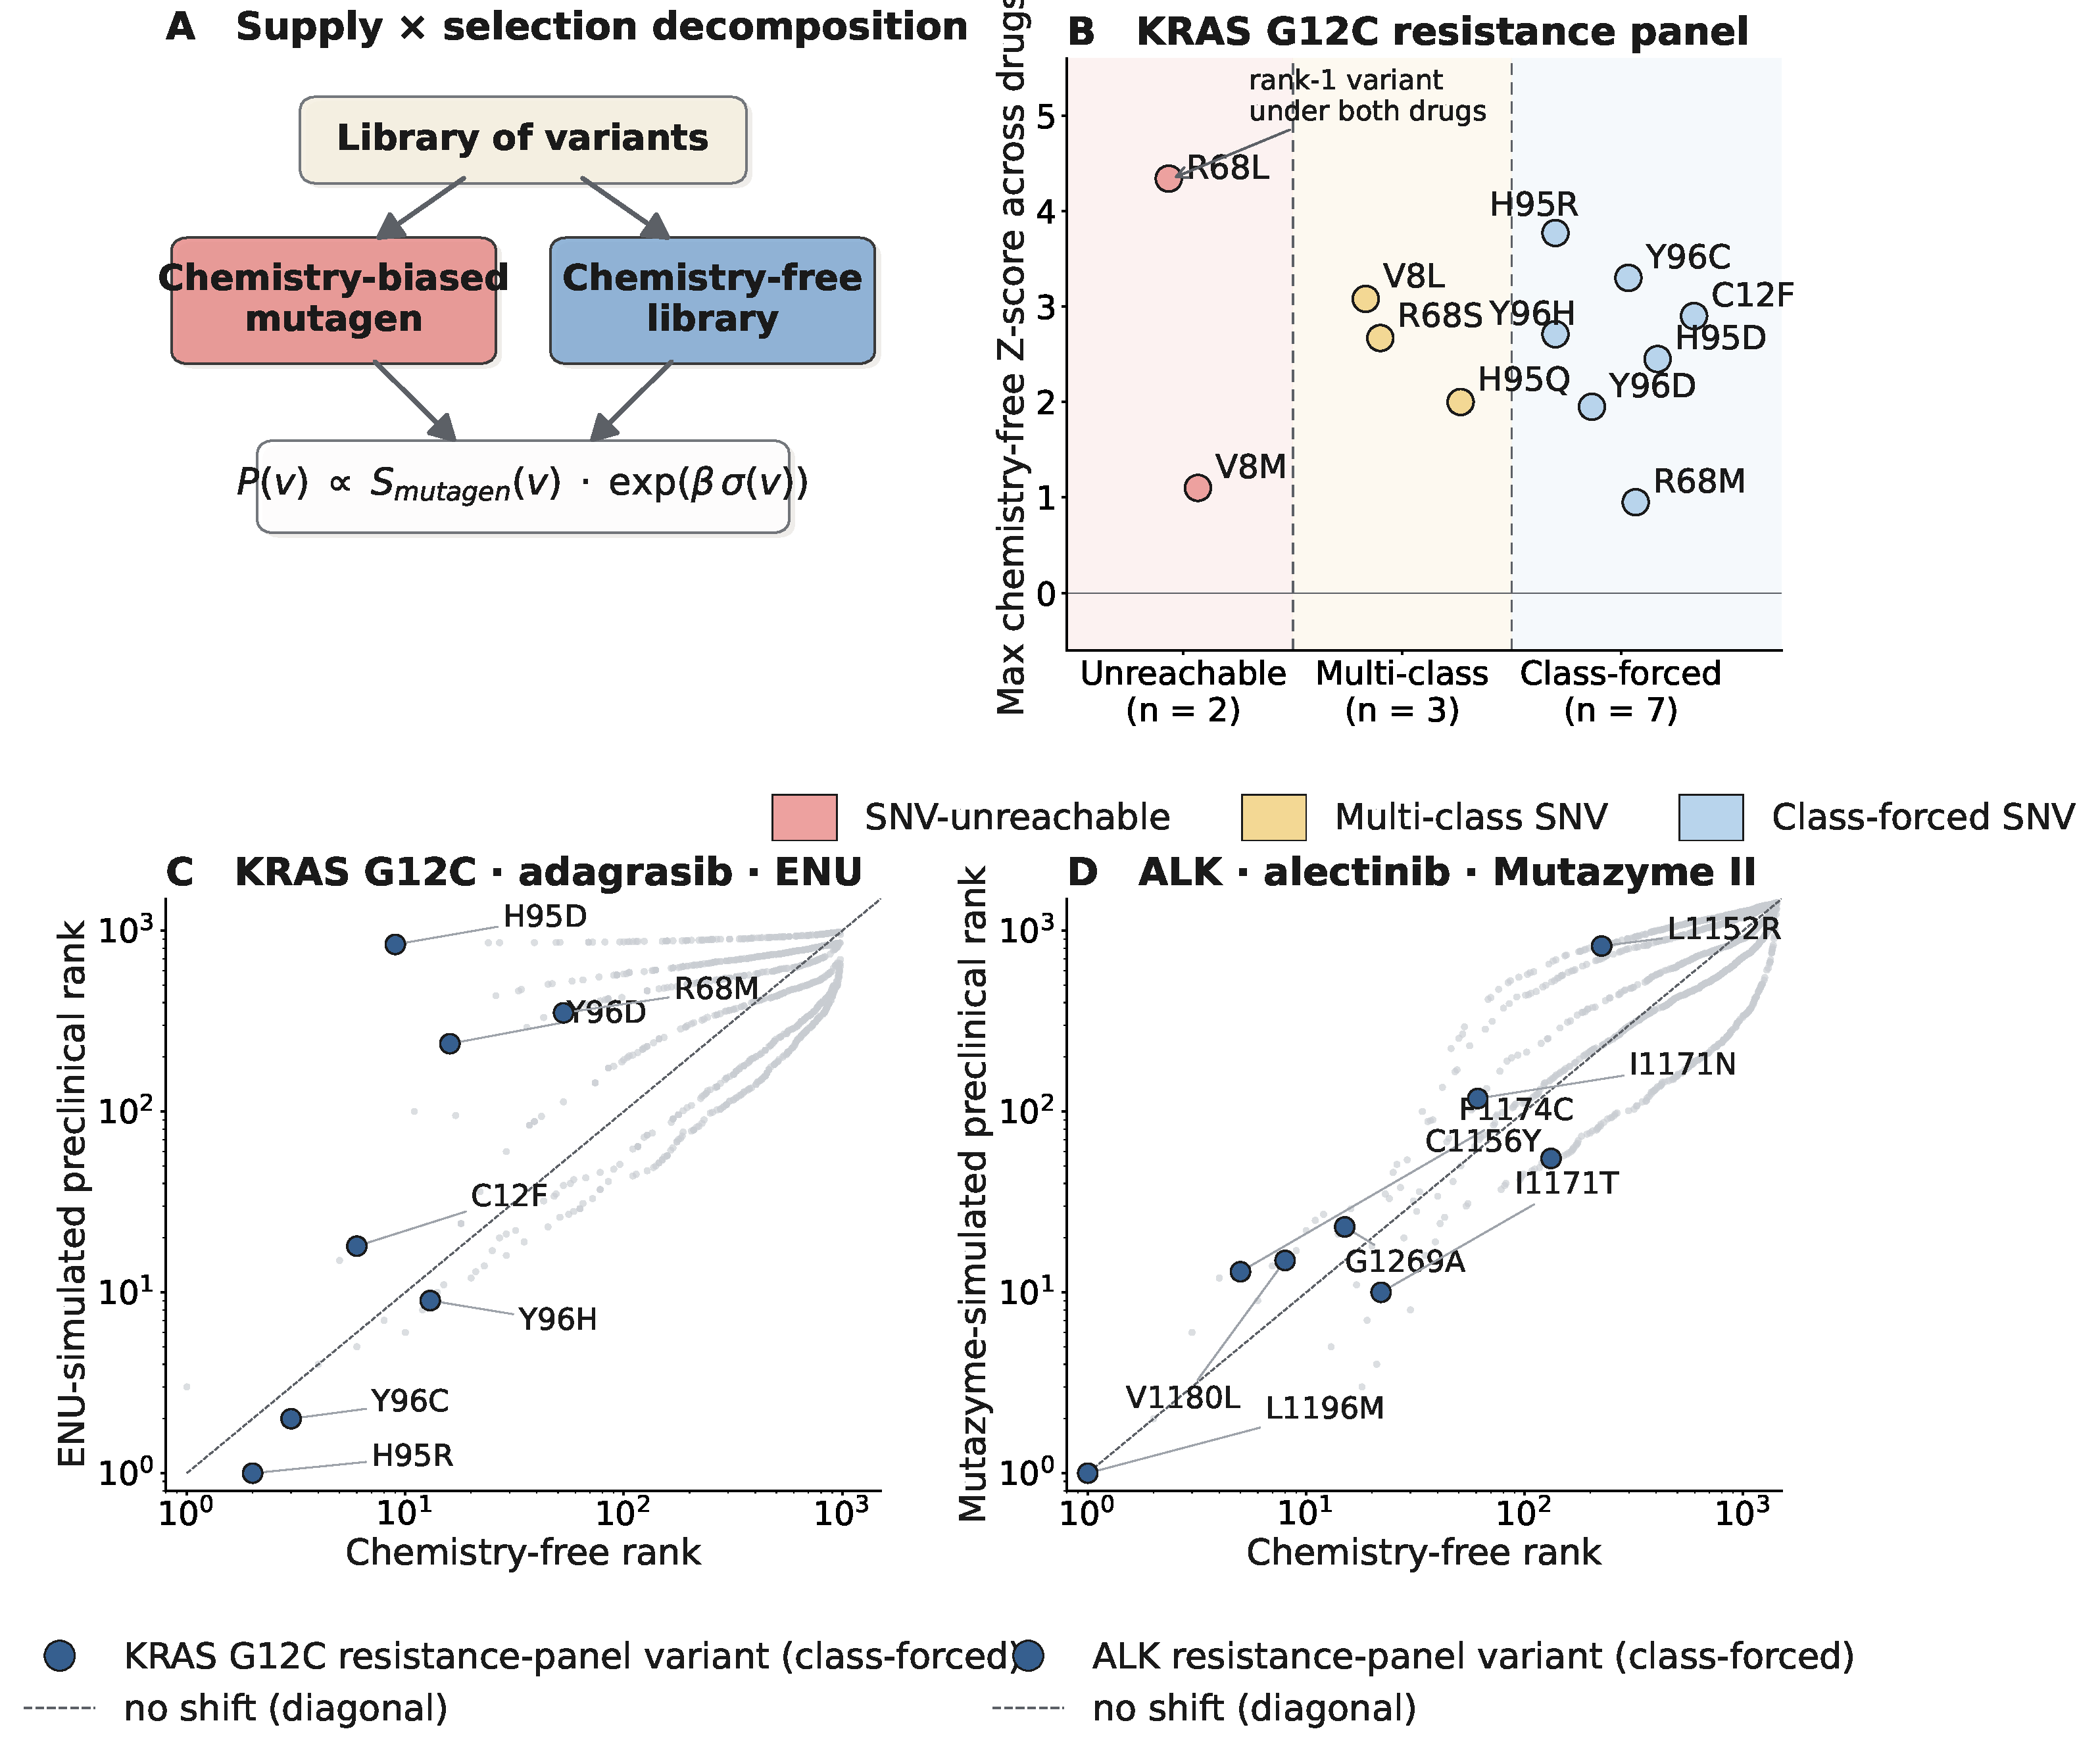
\includegraphics[width=\textwidth]{figure_1.pdf}
\caption{Chemistry-biased mutagens reorder and sometimes
forbid preclinical TKI-resistance rankings.
\textbf{A}, The supply $\times$ selection decomposition,
$P(v) \propto S_{\mathrm{mutagen}}(v)\cdot\exp(\beta\sigma(v))$.
\textbf{B}, The 12 composite KRAS G12C panel variants (Table~S1), binned by
single-nucleotide reachability from the wild-type codon; $y$, maximum
chemistry-free Z-score across sotorasib and adagrasib.
\textbf{C}, \textbf{D}, Simulated against chemistry-free rank, both axes
log scale, for KRAS G12C under ENU with adagrasib (1,205 variants
\citep{feng2022}) and for ALK under Mutazyme~II with alectinib (1,427
variants \citep{oh2026}); dashed line, no shift.}
\end{figure}
\begin{figure}[H]
\centering
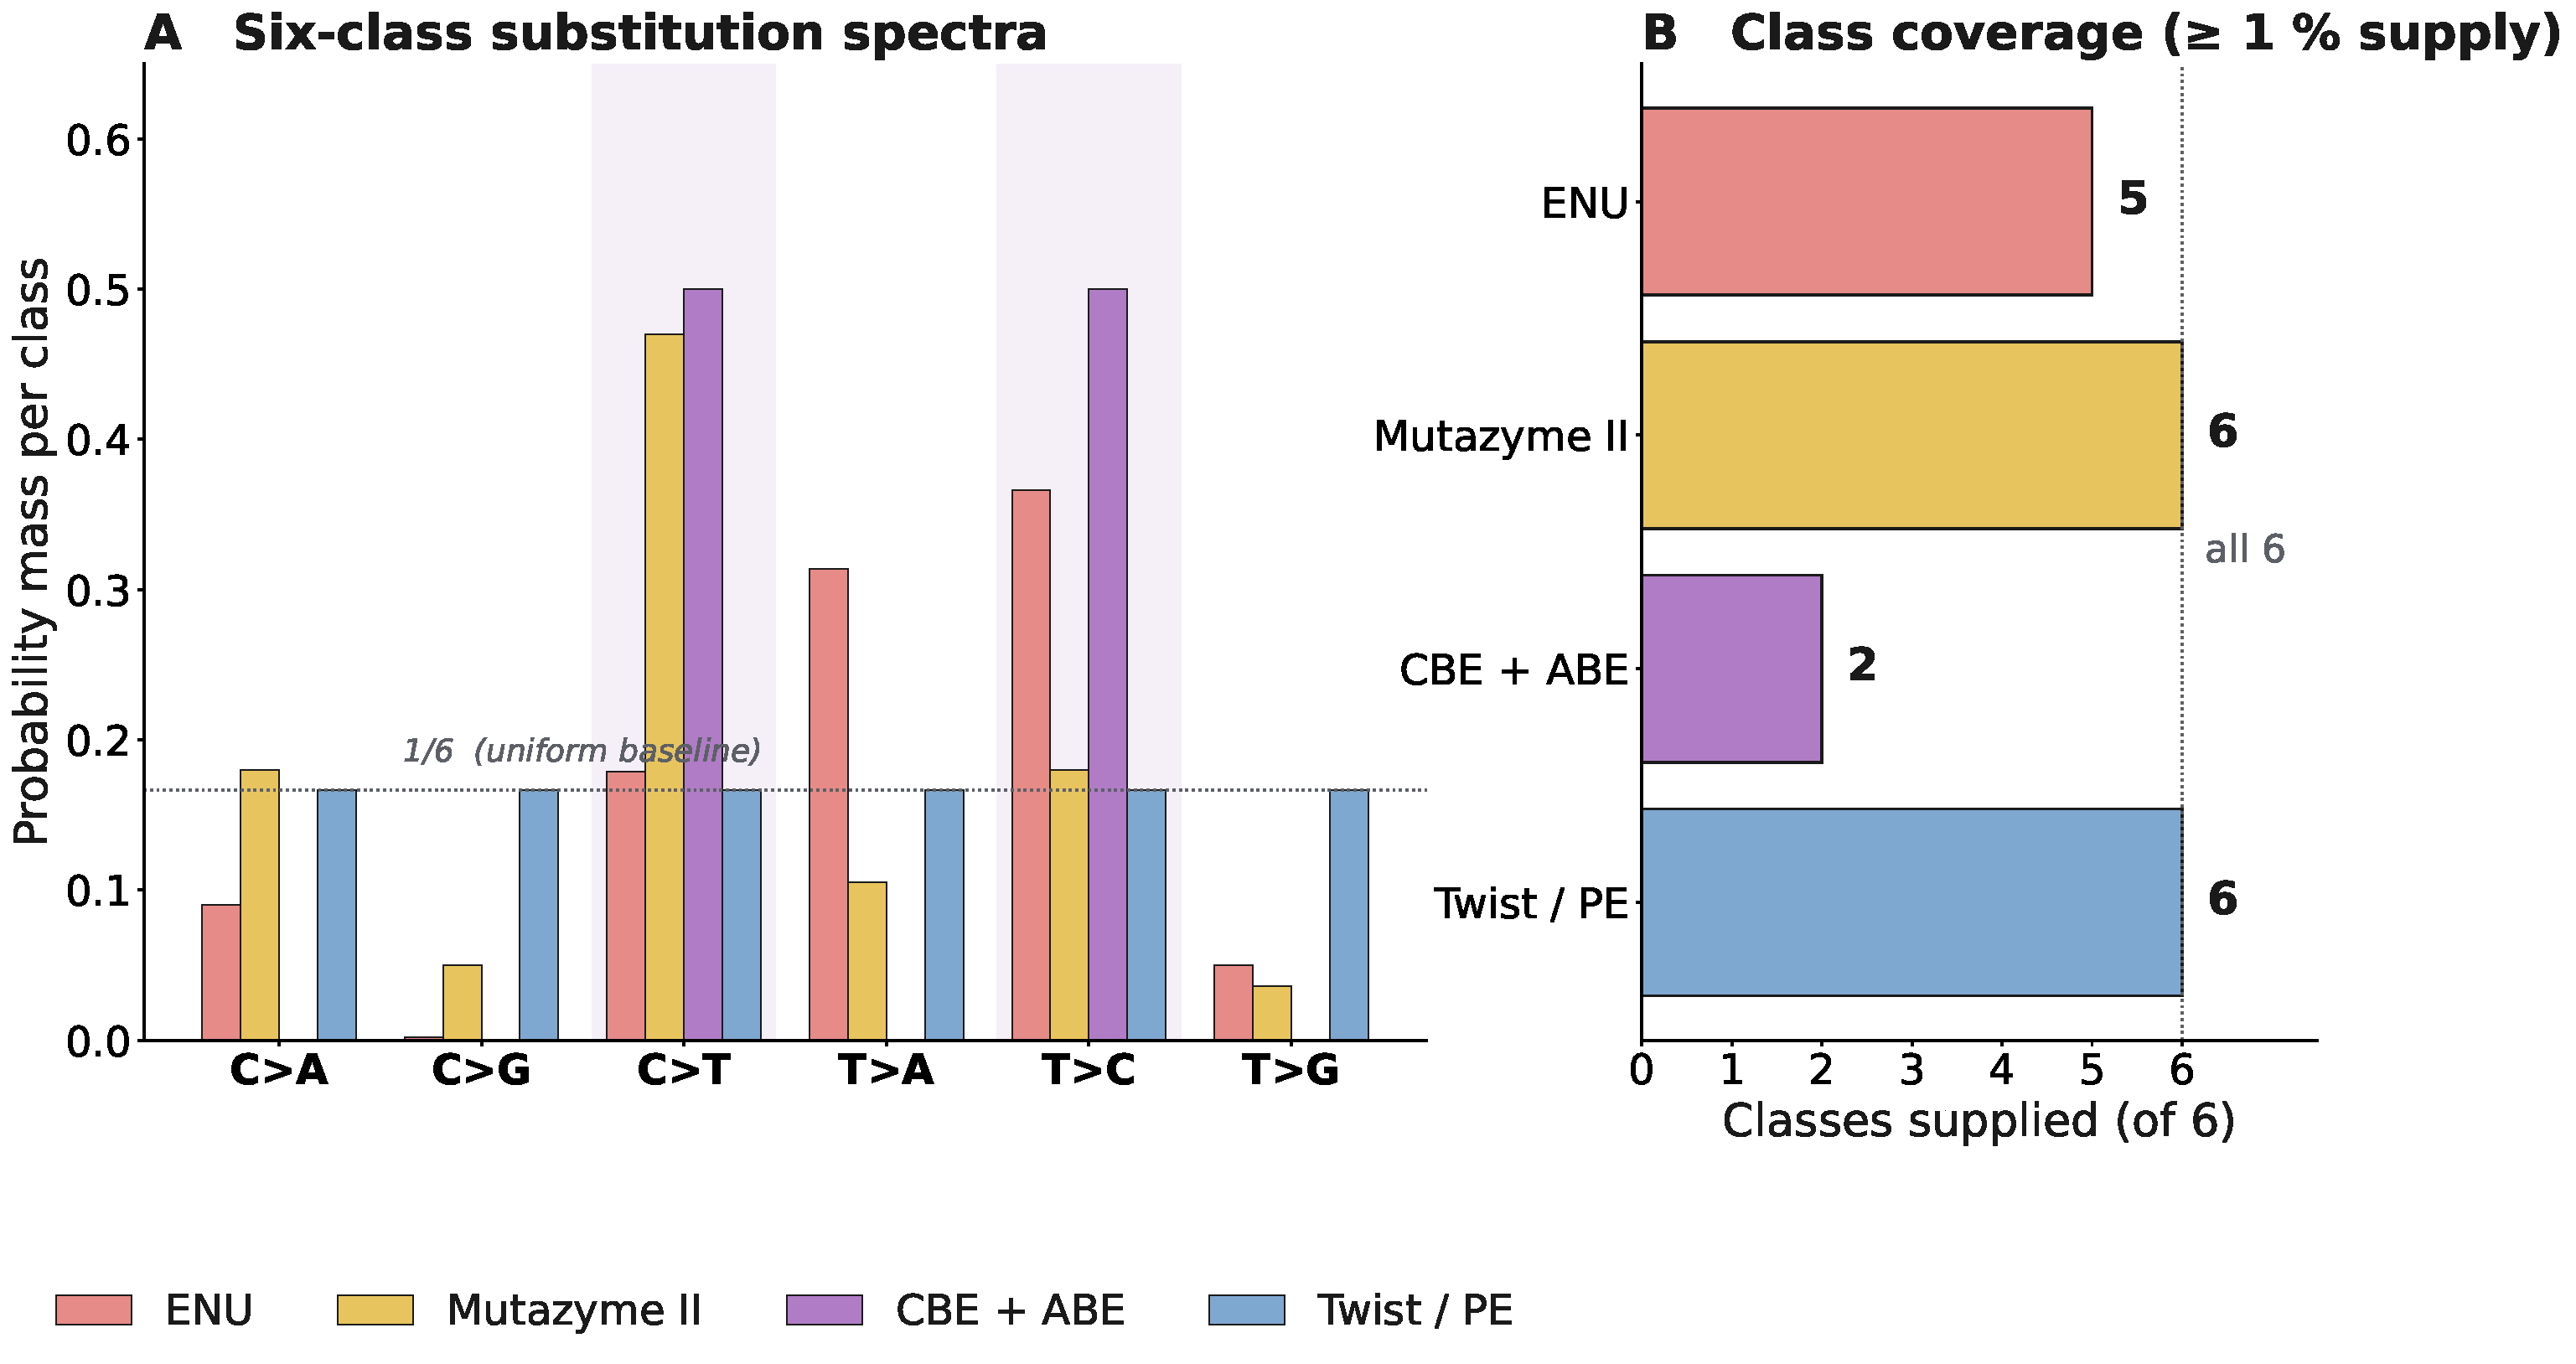
\includegraphics[width=\textwidth]{figure_2.pdf}
\caption{Mutagen chemistries used in current preclinical
TKI-resistance screens.
\textbf{A}, Six-class pyrimidine substitution spectra of ENU
\citep{arnold2012}, Mutazyme~II \citep{doi2022}, and combined CBE+ABE,
against the chemistry-free uniform baseline (1/6 per class, dotted). The
lavender band marks the two base-editing-reachable classes.
\textbf{B}, Number of classes each mutagen supplies at $\geq$ 1\%.}
\end{figure}
\begin{figure}[H]
\centering
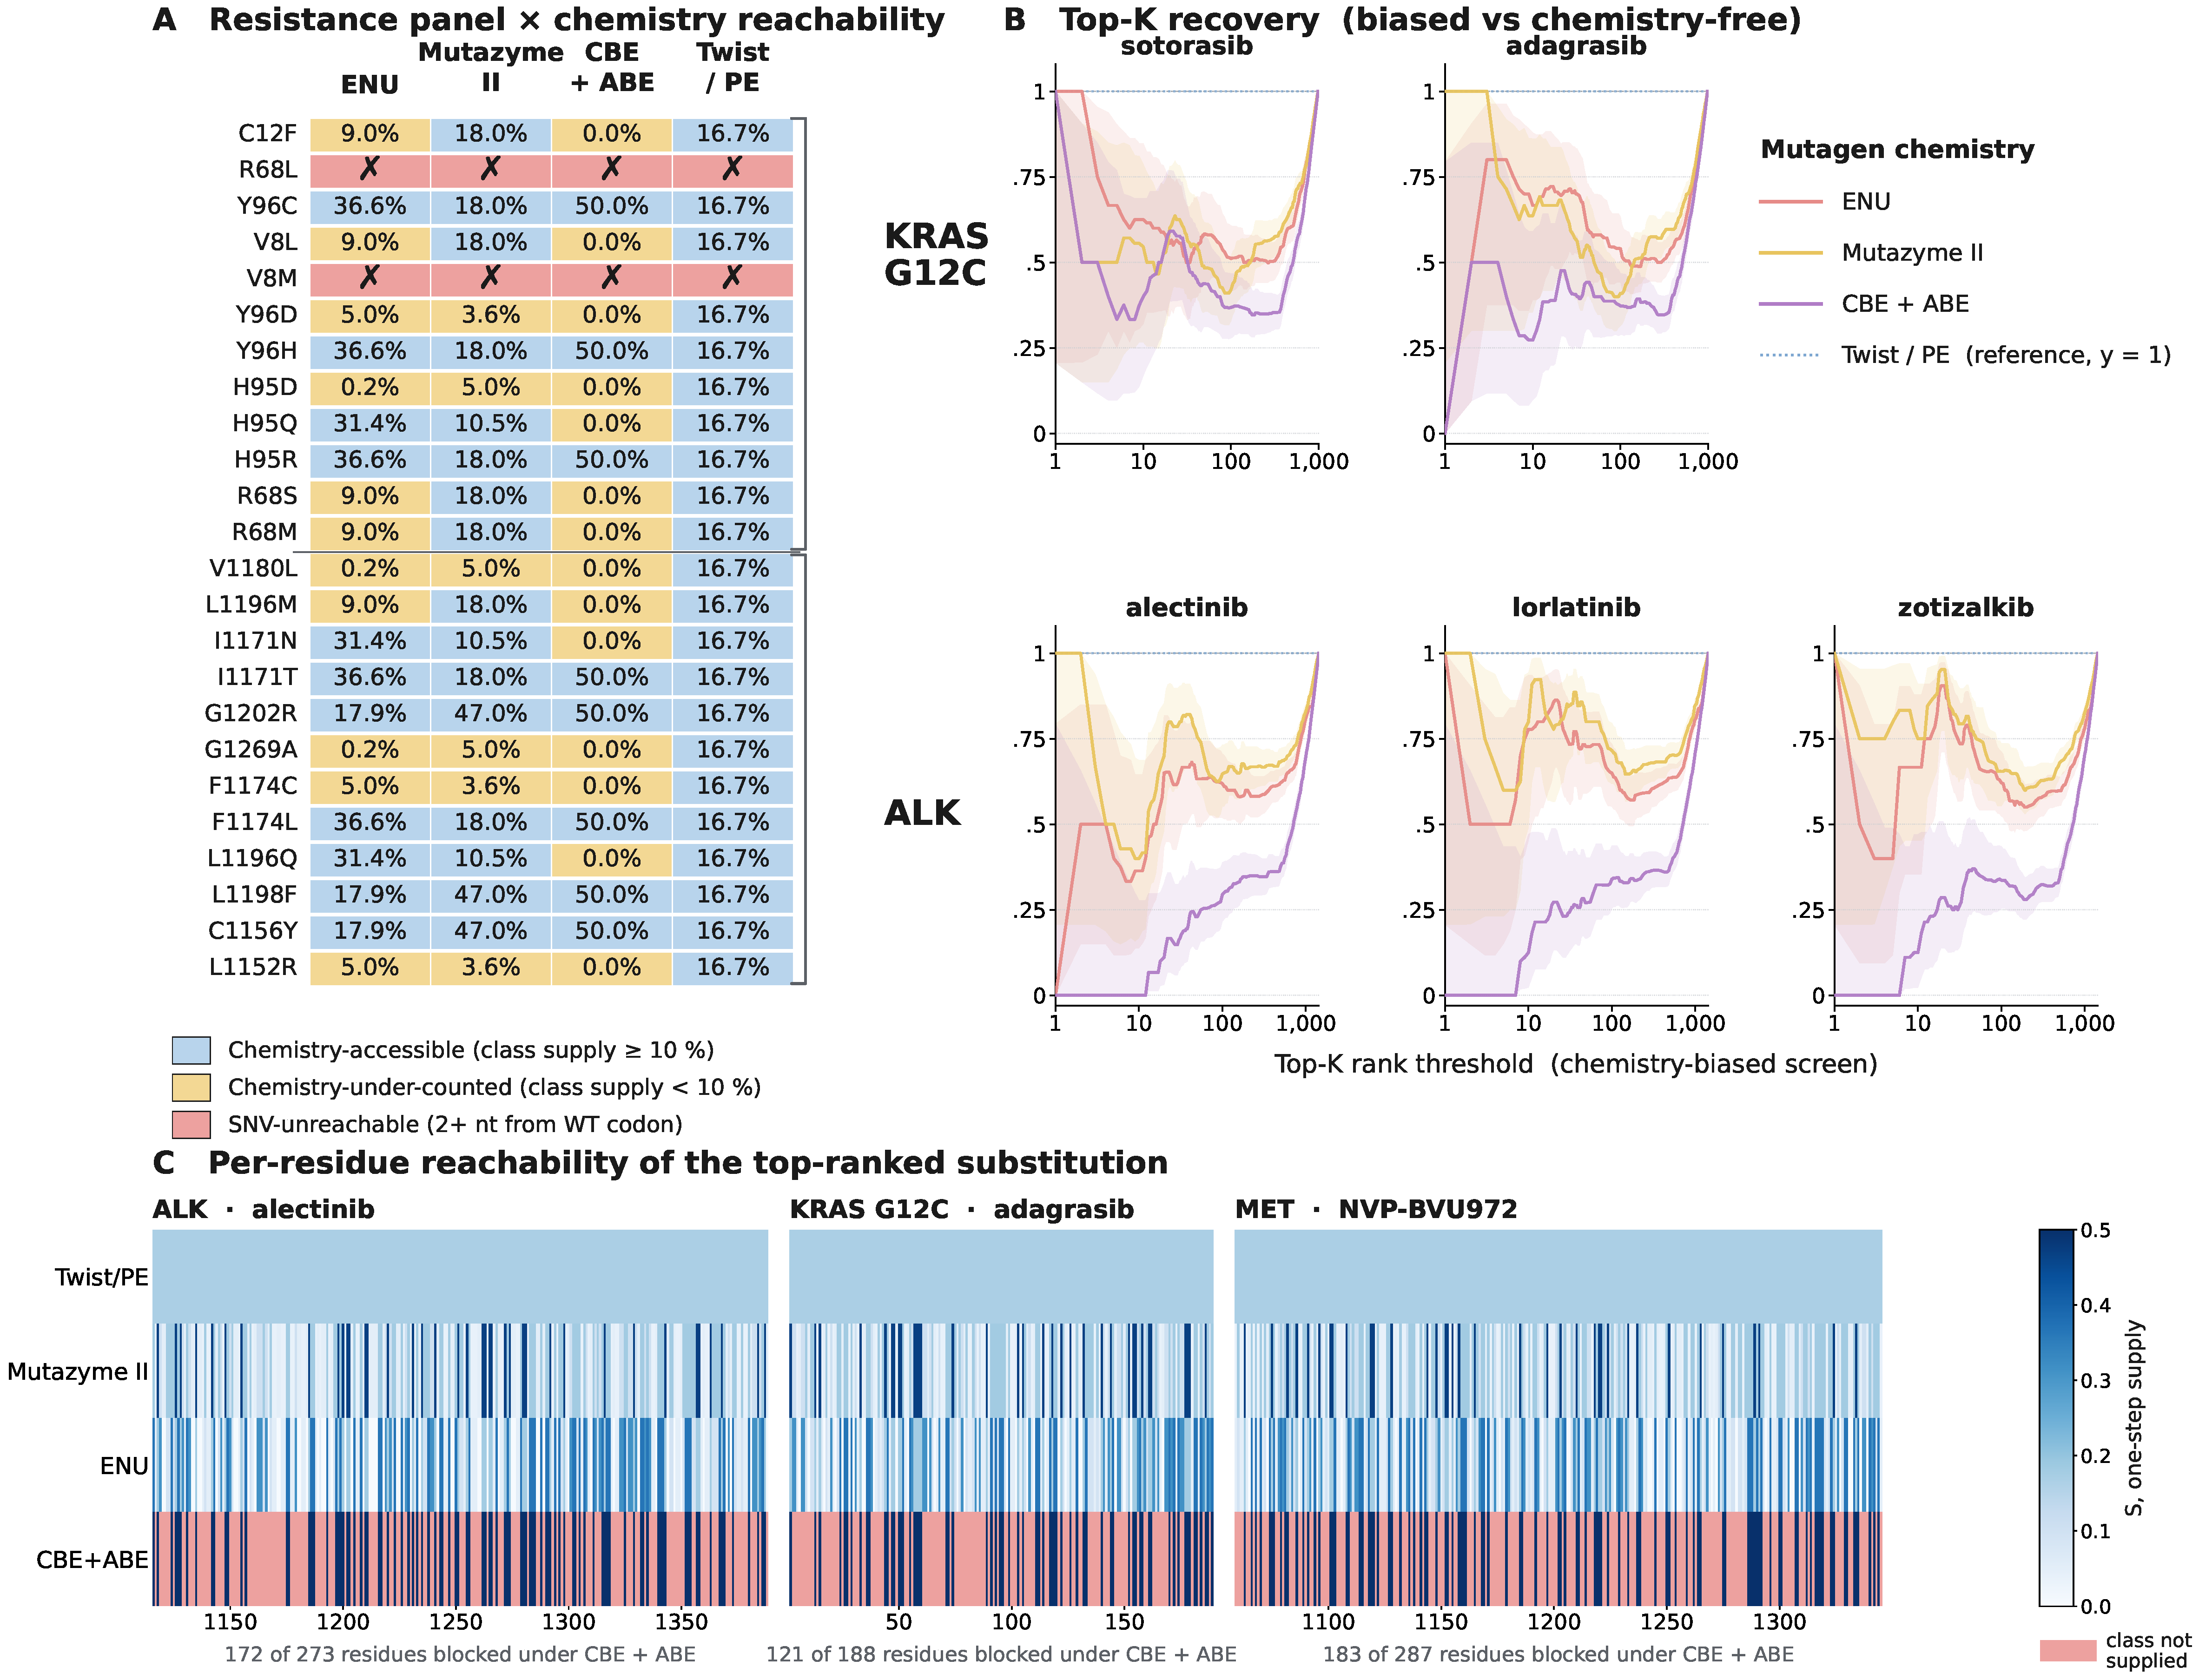
\includegraphics[width=\textwidth]{figure_3.pdf}
\caption{Chemistry blind-spots and recovery of priority
variants from the chemistry-free atlases.
\textbf{A}, Reachability of the 24 panel variants (KRAS G12C above the
divider, ALK below; Table~S1) under the four chemistries of
Table~\ref{tab:current-practice}. Blue, accessible (maximum class supply
$\geq$ 10\%); amber, under-counted ($<$ 10\%); red,
two-step from the wild-type codon. Labels give the maximum class supply.
\textbf{B}, Fraction of the chemistry-free top-$K$ also present in the
chemistry-biased top-$K$, one subpanel per gene and drug, with 95\% Wilson
bands and $K$ on a log scale. The chemistry-free reference is 1 by
construction (dotted). Colors as in Fig.~2A.
\textbf{C}, For every residue of each kinase domain, the one-step supply
each chemistry gives the substitution the chemistry-free atlas ranks
highest at that position (ALK with alectinib, KRAS G12C with adagrasib,
MET with NVP-BVU972; the other arms are in the interactive inventory).
The view covers class-forced substitutions only, so a chemistry counts as
blocked here just where its spectrum gives that class zero; variants
needing two or more nucleotide changes lie outside it by construction and
are reported in \S\ref{sec:kras-panel} and \S\ref{sec:met}. On that
scope ENU and Mutazyme~II block no residue in any of the three genes,
while CBE+ABE blocks 63\%--66\% of them.}
\end{figure}
\clearpage
\begin{figure}[H]
\centering
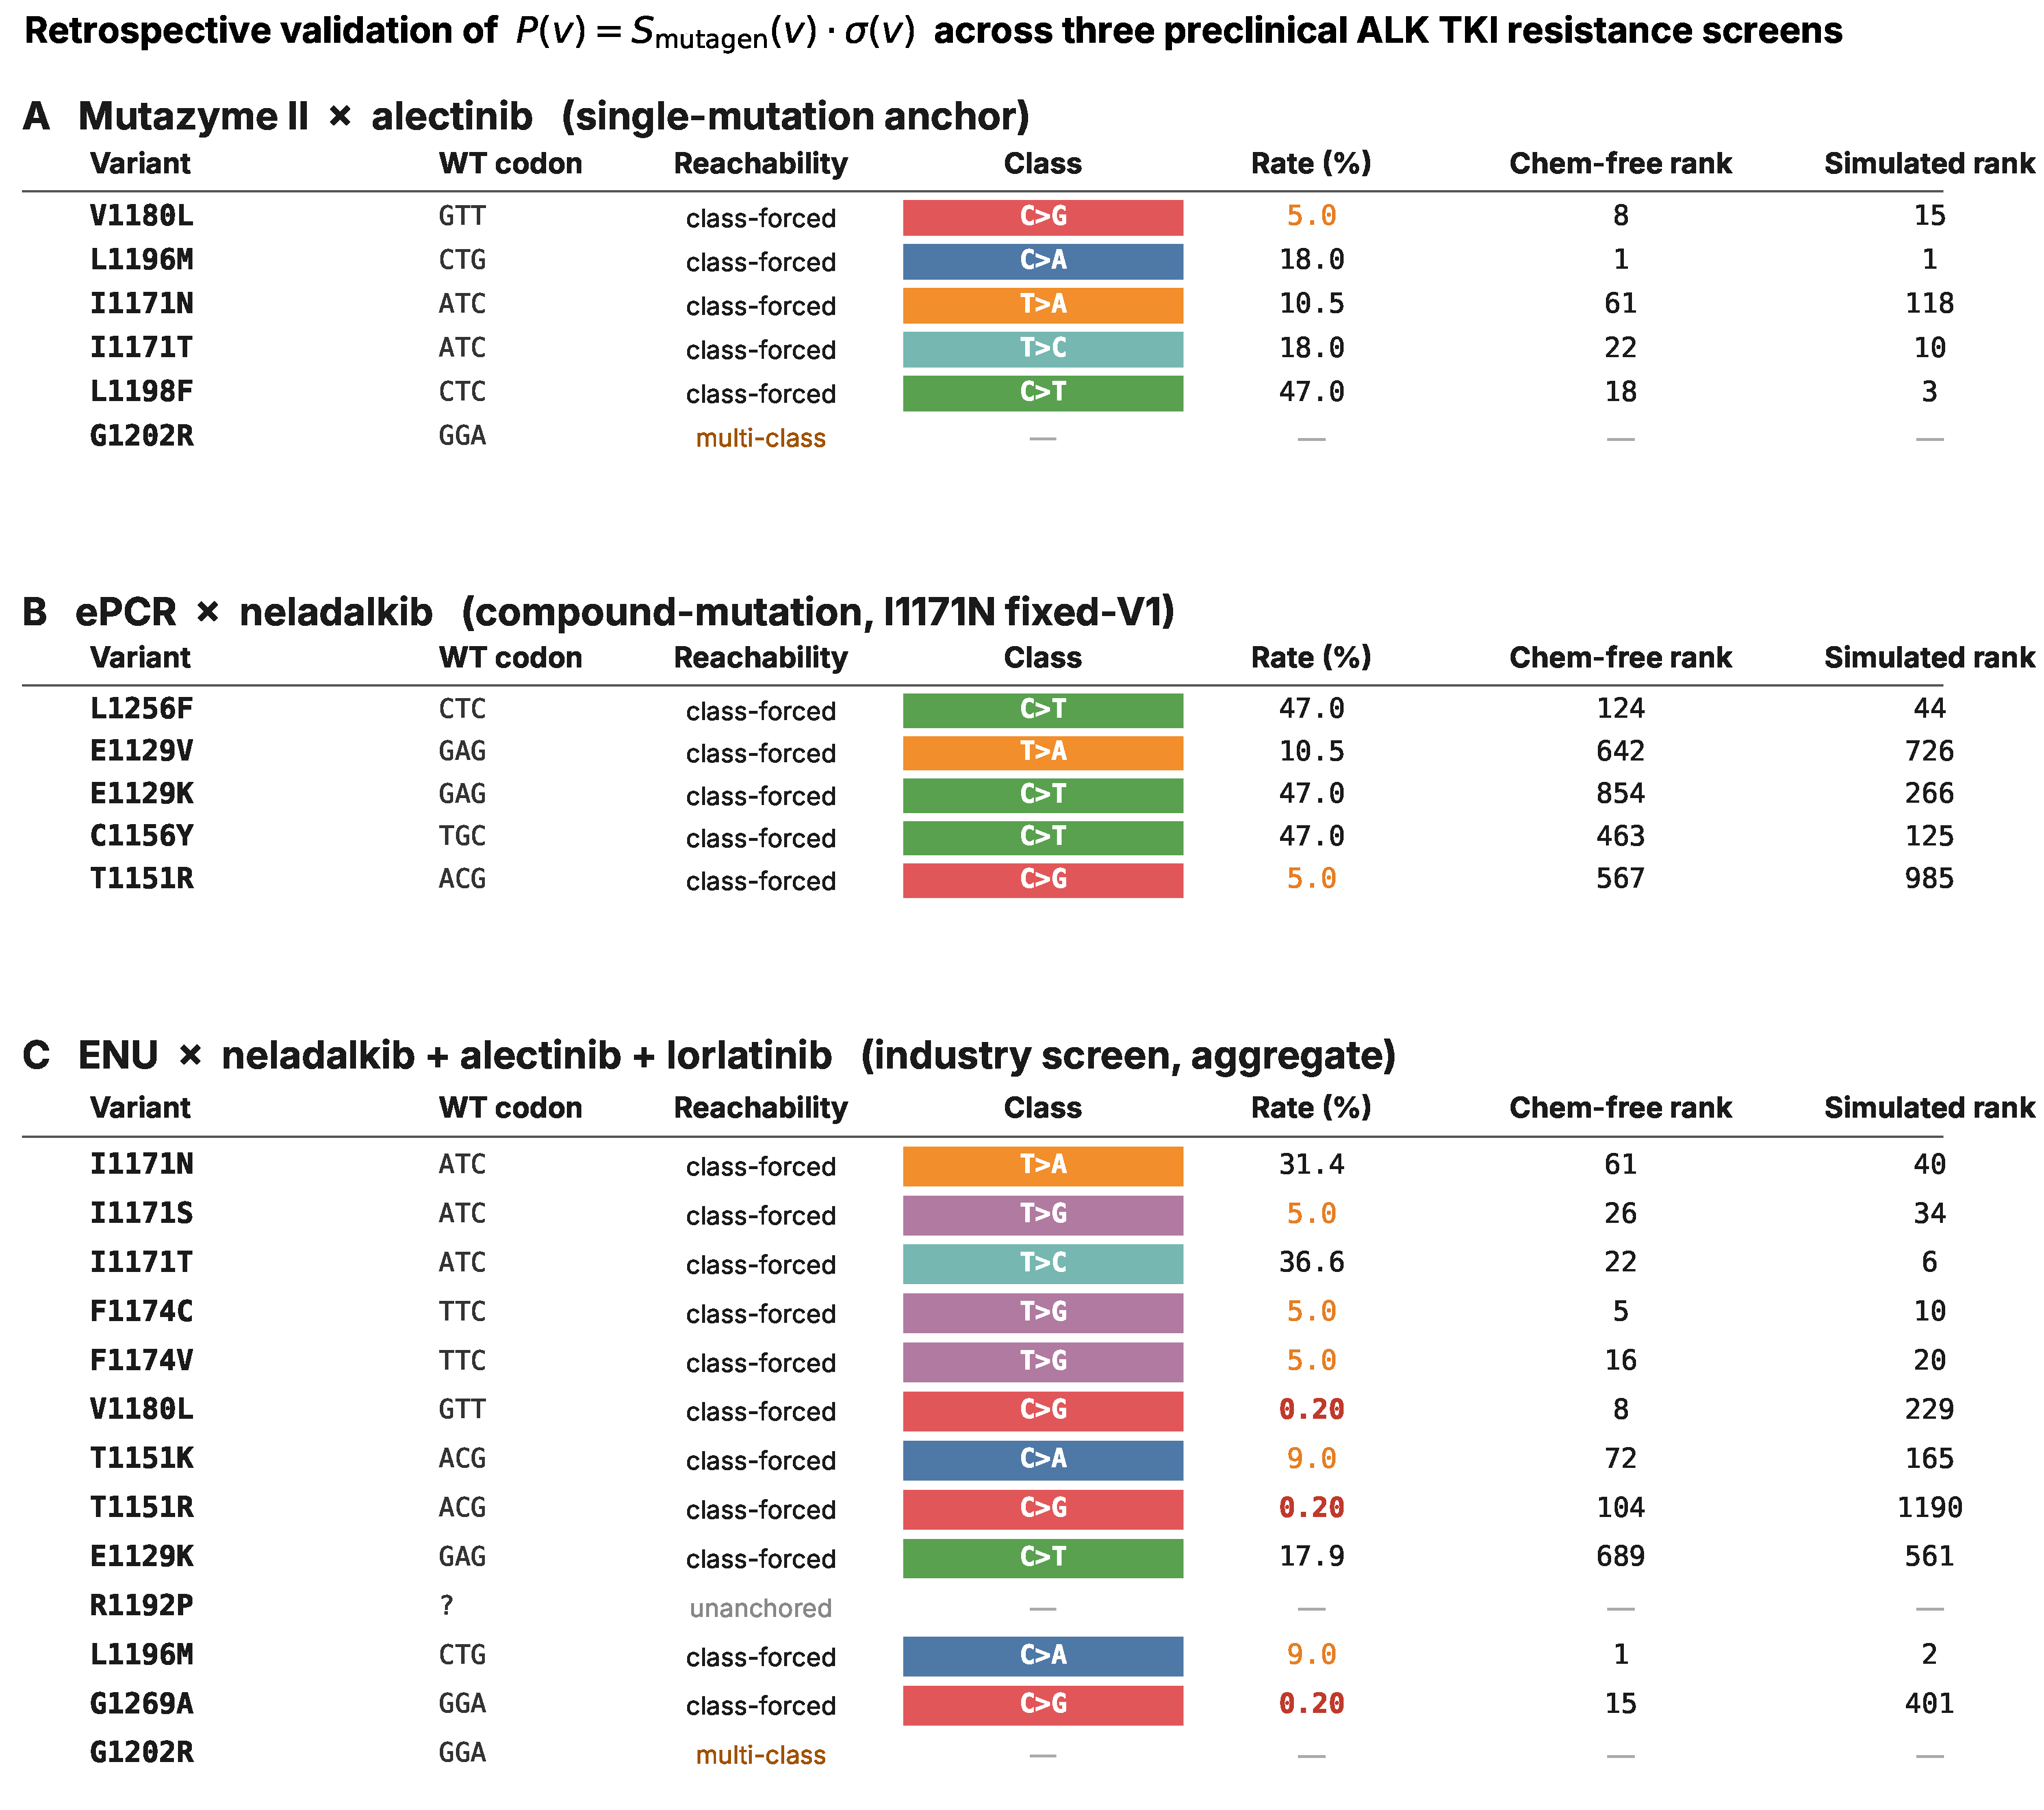
\includegraphics[width=\textwidth]{figure_4.pdf}
\caption{Retrospective validation of
$P(v) \propto S_{\mathrm{mutagen}}(v)\cdot \exp(\beta\sigma(v))$ across three
preclinical ALK TKI resistance screens. Each panel lists the screen's
observed variants with wild-type codon, reachability, forced substitution
class, class supply under the screen's mutagen, and chemistry-free against
simulated rank.
\textbf{A}, Mutazyme~II with alectinib \citep{doi2022}; six variants, five
class-forced (G1202R is multi-class and omitted).
\textbf{B}, ePCR neladalkib compound screen on an I1171N background
\citep{takei2025}; five V2 partners.
\textbf{C}, Industry ENU screen across alectinib, lorlatinib, and
neladalkib \citep{tangpeerachaikul2025}; thirteen aggregate hits, R1192P
outside the atlas residue window. Panels B and C use zotizalkib $\sigma$
as the fourth-generation proxy.}
\end{figure}

\clearpage
\begin{figure}[H]
\centering
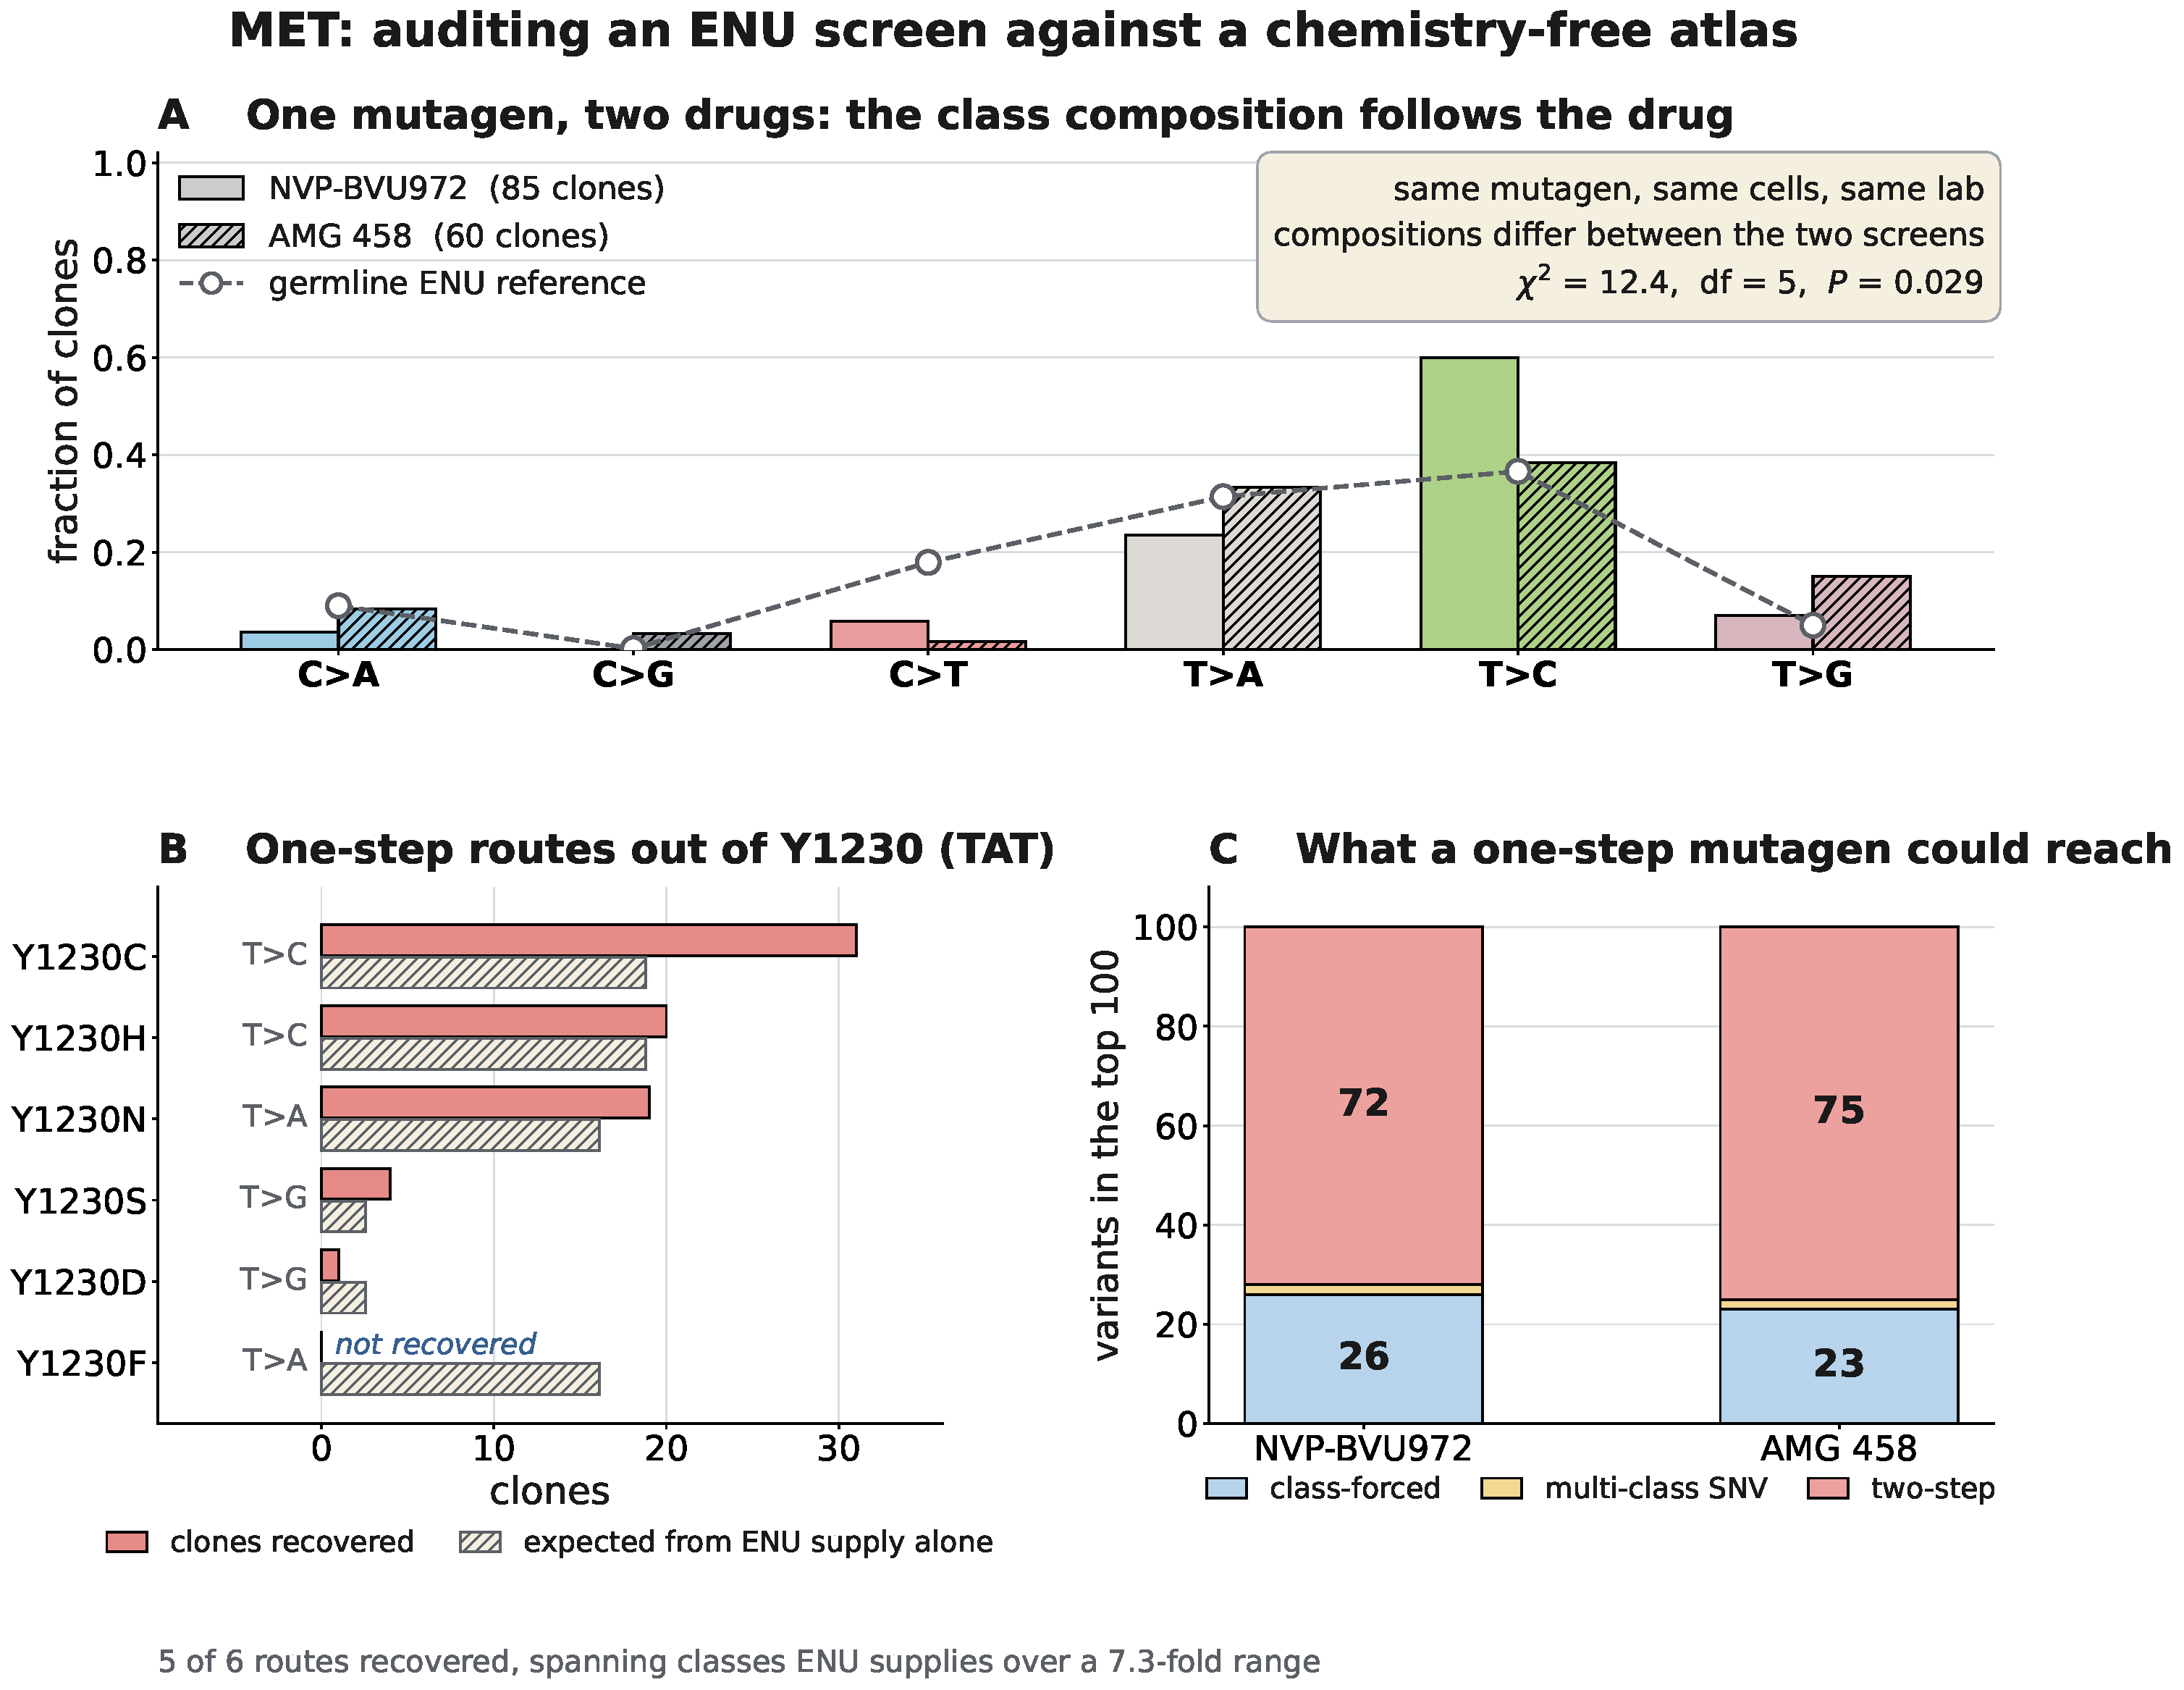
\includegraphics[width=\textwidth]{figure_5.pdf}
\caption{The MET audit. \textbf{A}, Six-class composition of the clones each
Tiedt screen recovered, taken from the nucleotide alterations that study
reports, against the germline ENU reference (dashed). One mutagen, one cell
line, one laboratory, two drugs. \textbf{B}, Every single-nucleotide missense
route out of the Y1230 wild-type codon TAT, with its substitution class, the
clones recovered, and what the ENU class supply alone predicts. \textbf{C},
Reachability of each drug's chemistry-free top 100 from the wild-type codon.}
\end{figure}

% ============================================================================
% REFERENCES
% ============================================================================
\clearpage
\bibliographystyle{unsrtnat}
\bibliography{refs}

\end{document}
